
\documentclass[
11pt, % The default document font size, options: 10pt, 11pt, 12pt
% oneside, % Two side (alternating margins) for binding by default, uncomment to switch to one side
english, % ngerman for German
singlespacing, % Single line spacing, alternatives: onehalfspacing or doublespacing
%draft, % Uncomment to enable draft mode (no pictures, no links, overfull hboxes indicated)
%nolistspacing, % If the document is onehalfspacing or doublespacing, uncomment this to set spacing in lists to single
%liststotoc, % Uncomment to add the list of figures/tables/etc to the table of contents
%toctotoc, % Uncomment to add the main table of contents to the table of contents
%parskip, % Uncomment to add space between paragraphs
% nohyperref, % Uncomment to not load the hyperref package
headsepline, % Uncomment to get a line under the header
]{MastersDoctoralThesis} % The class file specifying the document structure

\usepackage[utf8]{inputenc} % Required for inputting international characters
\usepackage[T1]{fontenc} % Output font encoding for international characters

\usepackage{palatino} % Use the Palatino font by default
\usepackage{xcolor}
\usepackage{graphicx}
\usepackage{hyperref}

\usepackage{algpseudocode}
\usepackage{algorithm2e}
\usepackage{pifont}
\usepackage{amsmath}
\usepackage[backend=bibtex,style=authoryear,natbib=true]{biblatex} % User the bibtex backend with the authoryear citation style (which resembles APA)
\renewcommand{\algorithmicrequire}{\textbf{Input:}}
\renewcommand{\algorithmicensure}{\textbf{Output:}}
\addbibresource{example.bib} % The filename of the bibliography

\usepackage[autostyle=true]{csquotes} % Required to generate language-dependent quotes in the bibliography
%----------------------------------------------------------------------------------------
%	MARGIN SETTINGS
%----------------------------------------------------------------------------------------

\geometry{
	paper=a4paper, % Change to letterpaper for US letter
	inner=2.5cm, % Inner margin
	outer=3.8cm, % Outer margin
	bindingoffset=2cm, % Binding offset
	top=1.5cm, % Top margin
	bottom=1.5cm, % Bottom margin
	%showframe,% show how the type block is set on the page
}

%----------------------------------------------------------------------------------------
%	THESIS INFORMATION
%----------------------------------------------------------------------------------------

\thesistitle{Knowledge Discovery From Academic Data Using Data Mining Technique} % Your thesis title, this is used in the title and abstract, print it elsewhere with \ttitle
\supervisor{Dr. ASM Latiful Hoque} % Your supervisor's name, this is used in the title page, print it elsewhere with \supname
\examiner{} % Your examiner's name, this is not currently used anywhere in the template, print it elsewhere with \examname
\degree{Undergraduate Thesis} % Your degree name, this is used in the title page and abstract, print it elsewhere with \degreename
\author{{Md.Mostafizur  \textsc{Rahman}}  {Sabid Bin Habib}} % Your name, this is used in the title page and abstract, print it elsewhere with \authorname
\addresses{} % Your address, this is not currently used anywhere in the template, print it elsewhere with \addressname

\subject{Knowledge Discovery Using Data Mining} % Your subject area, this is not currently used anywhere in the template, print it elsewhere with \subjectname
\keywords{{Data Mining}} % Keywords for your thesis, this is not currently used anywhere in the template, print it elsewhere with \keywordnames
\university{{Bangladesh University Of Engineering And Technology}} % Your university's name and URL, this is used in the title page and abstract, print it elsewhere with \univname
\department{{Department of Computer Science And Engineering}} % Your department's name and URL, this is used in the title page and abstract, print it elsewhere with \deptname
\group{} % Your research group's name and URL, this is used in the title page, print it elsewhere with \groupname
\faculty{} % Your faculty's name and URL, this is used in the title page and abstract, print it elsewhere with \facname

\hypersetup{pdftitle=\ttitle} % Set the PDF's title to your title
\hypersetup{pdfauthor=\authorname} % Set the PDF's author to your name
\hypersetup{pdfkeywords=\keywordnames} % Set the PDF's keywords to your keywords

\begin{document}

\frontmatter % Use roman page numbering style (i, ii, iii, iv...) for the pre-content pages

\pagestyle{plain} % Default to the plain heading style until the thesis style is called for the body content

%----------------------------------------------------------------------------------------
%	TITLE PAGE
%----------------------------------------------------------------------------------------

\begin{titlepage}
\begin{center}

\textsc{\LARGE \univname}\\[1.5cm] % University name
\textsc{\Large Undergraduate Thesis}\\[0.5cm] % Thesis type

\HRule \\[0.4cm] % Horizontal line
{\huge \bfseries \ttitle}\\[0.4cm] % Thesis title
\HRule \\[1.5cm] % Horizontal line
 
\begin{minipage}{0.4\textwidth}
\begin{flushleft} \large
\emph{Author:}\\
{\authorname} % Author name - remove the \href bracket to remove the link
\end{flushleft}
\end{minipage}
\begin{minipage}{0.4\textwidth}
\begin{flushright} \large
\emph{Supervisor:} \\
{\supname} % Supervisor name - remove the \href bracket to remove the link  
\end{flushright}
\end{minipage}\\[3cm]
 
\deptname\\[2cm] % Research group name and department name
 
{\large \today}\\[4cm] % Date
%\includegraphics{Logo} % University/department logo - uncomment to place it
 
\vfill
\end{center}
\end{titlepage}

%----------------------------------------------------------------------------------------
%	DECLARATION PAGE
%----------------------------------------------------------------------------------------

\begin{declaration}
\addchaptertocentry{\authorshipname}

\noindent We, Md.Mostafizur Rahman and Sabid Bin Habib, declare that this thesis titled, \enquote{\ttitle} and the work presented in it are my own. I confirm that:

\begin{itemize} 
\item This work was done wholly or mainly while in candidature for a research degree at this University.
\item Where any part of this thesis has previously been submitted for a degree or any other qualification at this University or any other institution, this has been clearly stated.
\item Where I have consulted the published work of others, this is always clearly attributed.
\item Where I have quoted from the work of others, the source is always given. With the exception of such quotations, this thesis is entirely my own work.
\item I have acknowledged all main sources of help.
\item Where the thesis is based on work done by myself jointly with others, I have made clear exactly what was done by others and what I have contributed myself.\\
\end{itemize}
 
\noindent Signed:\\
\rule[0.5em]{25em}{0.5pt} % This prints a line for the signature
 
\noindent Date:\\
\rule[0.5em]{25em}{0.5pt} % This prints a line to write the date
\end{declaration}


%----------------------------------------------------------------------------------------
%	ABSTRACT PAGE
%----------------------------------------------------------------------------------------

\begin{abstract}
\addchaptertocentry{\abstractname} % Add the abstract to the table of contents

The Thesis Abstract is written here (and usually kept to just this page). The page is kept centered vertically so can expand into the blank space above the title too\ldots

\end{abstract}

%----------------------------------------------------------------------------------------
%	ACKNOWLEDGEMENTS
%----------------------------------------------------------------------------------------

\begin{acknowledgements}
\addchaptertocentry{\acknowledgementname} % Add the acknowledgements to the table of contents

The acknowledgments and the people to thank go here, don't forget to include your project advisor\ldots

\end{acknowledgements}

%----------------------------------------------------------------------------------------
%	LIST OF CONTENTS/FIGURES/TABLES PAGES
%----------------------------------------------------------------------------------------
%\hypersetup{linkbordercolor=black}
\hypersetup{linkcolor=black}{
\tableofcontents % Prints the main table of contents
}
\listoffigures % Prints the list of figures

\listoftables % Prints the list of tables

\dedicatory{For/Dedicated to/To my\ldots} 

%----------------------------------------------------------------------------------------
%	THESIS CONTENT - CHAPTERS
%----------------------------------------------------------------------------------------

\mainmatter % Begin numeric (1,2,3...) page numbering

\pagestyle{thesis} % Return the page headers back to the "thesis" style

% Include the chapters of the thesis as separate files from the Chapters folder
% Uncomment the lines as you write the chapters

% Chapter 1

\chapter{Introduction} % Main chapter title

\label{Introduction} % For referencing the chapter elsewhere, use \ref{Chapter1} 

%----------------------------------------------------------------------------------------

% Define some commands to keep the formatting separated from the content 
\newcommand{\keyword}[1]{\textbf{#1}}
\newcommand{\tabhead}[1]{\textbf{#1}}
\newcommand{\code}[1]{\texttt{#1}}
\newcommand{\file}[1]{\texttt{\bfseries#1}}
\newcommand{\option}[1]{\texttt{\itshape#1}}

%----------------------------------------------------------------------------------------

Bangladesh University of Engineering and Technology(\textit{BUET}) is a renowned Technological University of \textit{Bangladesh}.Brilliant students around the country get admitted here for quality education.The huge amount of BIIS data represent the states of all the students of BUET in academic education.For a large educational institute like public university which generates large volumes of data,it requires an efficient way to apply data mining techniques for obtaining knowledge on the development and performance improvement of academic activities.The knowledge acquired from BIIS can be sufficient to look for answers to such questions as: which factors determine better or worse academic performance of students? Which factors in a Department can be crucial for quality education? Concepts and techniques of data mining are essential to discover the hidden knowledge from large datasets \cite{concepts} .

\section{Problem Definition}
Every year BUET enrolls almost 1000 brilliants Engineering minded student into 11 different departments from all over the country and simultaneously almost 1000 students graduate from BUET.The BIIS data holds all the academic information of individual student in detail.Statistics from BIIS data shows that academic performance of a student varies from department to department.After close observation,it has been revealed that department might not be the only factor behind the performance of a student.There might be some other reasons such as CGPA, Hall Status,Gender,Class Test Marks,Attendance Status which affect a students performance.Only statistical analysis is not sufficient for finding out the knowledge from the BIIS data.The hidden knowledge inside the institutional academic and personal data of students is necessary to find out the possible effects on any students academic performance.That is why knowledge discovery and data mining from academic data is essential for educational institution like BUET to improve academic performance of students as well as reshaping the decision makings for the betterment of the institution.
Data mining techniques are very effective for discovering the hidden knowledge from educational data and applying it properly for the decision making.But all the data mining techniques can not be applied directly on academic data because of complex structure.This requires rigorous preprocessing.Bringing all the relevant data in a useful scope and applying classification methods on them are other problems of this research. 
\section{Scope of the Work}
The BIIS data represents the detailed academic performance of an individual student throughout the undergrad period. These students are under 5 different faculties.These five faculties are Faculty of Architecture \& Planning,Faculty of Civil Engineering,Faculty of Mechanical Engineering,Faculty of Engineering and Faculty of Electrical \& Electronic Engineering.There are 11 different departments under these faculties which are Department of Electrical \& Electronic Engineering, Department of Computer Science \& Engineering, Department of Civil Engineering,Department of Mechanical Engineering,Department of Architecture,Department of Water Resource Engineering,Department of Naval Architecture \& Marine Engineering,Department of Chemical Engineering,Department of Materials \& Metallurgical Engineering,Department of Urban \& Regional Planning and Department of Industrial \& Production Engineering. \cite{buet}
The scope of knowledge discovery from BIIS data is immense in context of undergraduate students.In this research BIIS data of 10 already graduated batches have been used which represents almost 10 thousand students maintaining the privacy of the data. No current student has been brought under this research. 
\section{Objectives}
Every year, a number of brilliant minded students are admitted into BUET,but at the end of their academic period,all of them can not utilize the full potential,it affects their academic performance.The main objectives of this research study are
\begin{itemize}
\item To find out the effect of different factors to the performance of a student.
\item To discover knowledge of students’ academic performance and personal 
statistics through the impact of different assessment and factors e.g. Class 
Test, Attendance, CGPA, Credit Completion etc.
\item Compare the impact of different factors e.g. Hall Status, Gende , Class 
Test, Attendance, Departments on the academic performances of a 
student
\end{itemize}
 
\section{Thesis organization}
We have developed a technique to discover knowledge using ID3 classification algorithm from institutional data of students who have completed their undergraduate in the department of CSE,BUET.\\All the literature studies e.g., preprocessing of raw data, prelimineries of Knowledge Discovery and Data Mining, Building decision tree, ID3 algorithm and related works have been elaborated in chapter 2.\\Description of the raw academic and analysis have been described in chapter 3.Basically,the raw BIIS data is not suitable for implementation of necessary procedures,the status of the data has been elaborated in chapter 3.\\
The existing raw data needs to be rigorously preprocessed before the implementation of classification.The step by step methodologies and the result of this preprocess has been described in chapter 4.\\
On chapter 5,the implementation of ID3 classification algorithm on the test data using training set has been elaborated.The result of the procedures taken has also been depicted in this section in detail.\\Finally,we have illustrated the summary of the findings along with quantitative analysis.We ave also encompassed the scope of the extension of this research work by illustrating some significant future works in chapter 6.  





% Chapter 2



\chapter{Literature Study} % Main chapter title

\label{Literature Study} % For referencing the chapter elsewhere, use \ref{Chapter1} 

%----------------------------------------------------------------------------------------

% Define some commands to keep the formatting separated from the content 

%----------------------------------------------------------------------------------------

\section{Knowledge Discovery Steps}
Knowledge Discovery is the non-trivial process of identifying valid, novel, potentially useful, and ultimately understandable patterns in data \\\cite{knowledge discovery}. With the emphasis on collecting data increasing around the world, there is an urgent need for a new generation of different techniques, methods and algorithms to assist researchers, analysts, decision makers and managers in extracting useful patterns from the rapidly growing volumes of data. These techniques and tools are the subject of the emerging field of knowledge discovery in databases .Knowledge Discovery and Data Mining  is an interdisciplinary area focusing upon methodologies for extracting useful knowledge from data.Knowledge Discovery and Data Mining is an interdisciplinary area focusing upon methodologies for extracting useful knowledge from data.According to \cite{IBM}, Though Knowledge Discovery is used synonymously to represent data mining, both these are actually different. Some preprocessing steps before data mining and post processing steps after data mining are to be completed to transform the raw data as useful knowledge. \newline
Knowledge Discovery is an iterative process that transforms raw data into useful information. Different steps of Knowledge Discovery in Databases are discussed in \cite{kddsteps}.

\begin{figure}
\centering
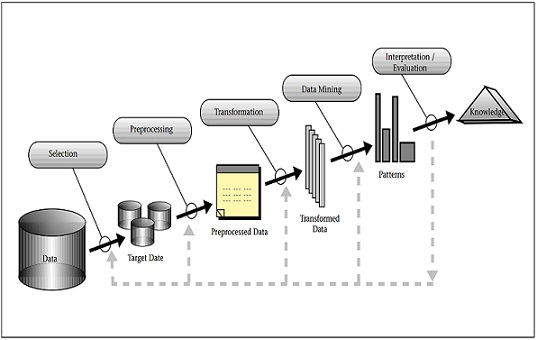
\includegraphics{Figures/kdsteps.jpg}
\decoRule
\caption{Knowledge discovery steps}
\label{fig:kdsteps}
\end{figure}



Figure \ref{fig:kdsteps} shows the general process of knowledge discovery.

\subsection{Understanding the Application Domain}
The first step is understanding requirements.It is needed to have a clear understanding about the application domain and your objectives.It should be also known whether the data is going to be described or information is predicted.
\subsection{Selection of Dataset}
Data mining is done on current or past records. Thus,a data set or subset of data should be selected, in other words data samples, on which you need to perform data analysis and get useful knowledge.There should be enough quantity of data to perform data mining.
\subsection{Data Cleaning}
Data cleaning is the step where noise and irrelevant data are removed from the large data set. This is a very important preprocessing step because the outcome would be dependent on the quality of selected data. As part of data cleaning, duplicate records might have to be removed, logically correct values for missing records might have to be entered, unnecessary data fields might have to be removed, data format standardized, update data in a timely manner and so on.
\subsection{Data transformation}
With the help of dimensionality reduction or transformation methods, the number of effective variables is reduced and only useful features are selected to depict data more efficiently based on the goal of the task. In short, data is transformed into appropriate form making it ready for data mining step.
\subsection{Finding interesting features in the database}
This step is extremely important in the field of International Studies. Researchers and practitioners with different backgrounds and different languages may work on a given database, getting different results. Each group may consider different attributes in doing so.
\subsection{Selection of data mining task}
Based on the objective of data mining, appropriate task is selected. Some common data mining tasks are classification, clustering, association rule discovery, sequential pattern discovery, regression and deviation detection. You can choose any of these tasks based on whether you need to predict information or describe information.
\subsection{Selection of Data mining method}
Appropriate method(s) is to be selected for looking for patterns from the data. You need to decide the model and parameters that might be appropriate for the method. Some popular data mining methods are decision trees and rules, relational learning models, example based methods etc.
\subsection{Data mining}
Data mining is the actual search for patterns from the data available using the selected data mining method.
\subsection{Pattern evaluation}
This is a post processing step in KDD which interprets mined patterns and relationships. If the pattern evaluated is not useful, then the process might again start from any of the previous steps, thus making KDD an iterative process.
\subsection{Knowledge consolidation}
This is the final step in Knowledge Discovery. The knowledge discovered is consolidated and represented to the user in a simple and easy to understand format. Mostly, visualization techniques are being used to make users understand and interpret information. \newline

Though these are the main steps in any Knowledge Discovery process, some of the steps could be done combined during the actual process.  For example, considering the convenience, data selection and data transformation can be combined together. Even after presenting knowledge to the user, new data can be added to the data set or mining can be further refined or a different data mining method can be chosen to get more accurate results. Thus, Knowledge Discovery is completely an iterative process.


%----------------------------------------------------------------------------------------

\section{Data Mining Concepts}

\paragraph{}
Data mining is the process of discovering interesting patterns and knowledge from large amounts of data. The
data sources can include databases, data warehouses, the Web, other information repositories, or data that are
streamed into the system dynamically.
\begin{figure}
   \centering
  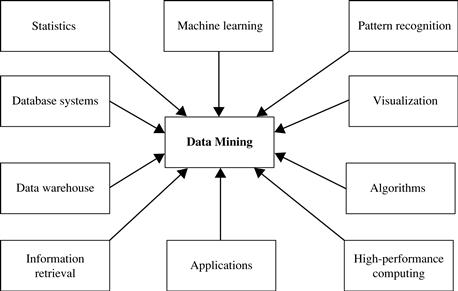
\includegraphics[width=\linewidth]{Figures/datamining.jpg}
  \decoRule
  \caption[Data Mining]{Data Mining Concept}
  \label{fig:datamining}
\end{figure}

Figure \ref{fig:datamining} shows the general parts of data mining.
As a general technology, data mining can be applied to any kind of data as long as the data are meaningful for a
target application. The most basic forms of data for mining applications are database data, data warehouse data, and transactional data.
\subsection{Database Data}
\paragraph{}
A database system, also called a database management system (DBMS), consists of a collection of
interrelated data, known as a database, and a set of software programs to manage and access the data. The
software programs provide mechanisms for defining database structures and data storage; for specifying and
managing concurrent, shared, or distributed data access; and for ensuring consistency and security of the
information stored despite system crashes or attempts at unauthorized access.
\paragraph{}
A relational database is a collection of tables, each of which is assigned a unique name. Each table consists of
a set of attributes (columns or fields) and usually stores a large set of tuples (records or rows). Each tuple in a
relational table represents an object identified by a unique key and described by a set of attribute values. A
semantic data model, such as an entity-relationship (ER) data model, is often constructed for relational
databases. An ER data model represents the database as a set of entities and their relationships.

\subsection{Data Warehouses}
\paragraph{}
A data warehouse is usually modeled by a multidimensional data structure, called a data cube, in which each
dimension corresponds to an attribute or a set of attributes in the schema, and each cell stores the value of
some aggregate measure such as count or sum. A data cube provides a multidimensional view of
data and allows the precomputation and fast access of summarized data.

\subsection{Transactional Data}
\paragraph{}
In general, each record in a transactional database captures a transaction, such as a customer\'s purchase, a
flight booking, or a user's clicks on a web page. A transaction typically includes a unique transaction identity
number (trans\_ID) and a list of the items making up the transaction, such as the items purchased in the
transaction. A transactional database may have additional tables, which contain other information related to the
transactions, such as item description, information about the salesperson or the branch, and so on.


\subsection{Other Kinds of Data}
\paragraph{}
Besides relational database data, data warehouse data, and transaction data, there are many other kinds of data
that have versatile forms and structures and rather different semantic meanings. Such kinds of data can be seen
in many applications: time-related or sequence data (e.g., historical records, stock exchange data, and timeseries and biological sequence data), data streams (e.g., video surveillance and sensor data, which are
continuously transmitted), spatial data (e.g., maps), engineering design data (e.g., the design of buildings,
system components, or integrated circuits), hypertext and multimedia data (including text, image, video, and
audio data), graph and networked data (e.g., social and information networks), and the Web (a huge, widely
distributed information repository made available by the Internet). These applications bring about new
challenges, like how to handle data carrying special structures (e.g., sequences, trees, graphs, and networks)
and specific semantics (such as ordering, image, audio and video contents, and connectivity), and how to mine
patterns that carry rich structures and semantics.
\\
Various kinds of knowledge can be mined from these kinds of data. Here, we list just a few. Regarding
temporal data, for instance, we can mine banking data for changing trends, which may aid in the scheduling of
bank tellers according to the volume of customer traffic. Stock exchange data can be mined to uncover trends
that could help you plan investment strategies. \\We could
mine computer network data streams to detect intrusions based on the anomaly of message flows, which may
be discovered by clustering, dynamic construction of stream models or by comparing the current frequent
patterns with those at a previous time. With spatial data, we may look for patterns that describe changes in
metropolitan poverty rates based on city distances from major highways. The relationships among a set of
spatial objects can be examined in order to discover which subsets of objects are spatially autocorrelated or
associated. By mining text data, such as literature on data mining from the past ten years, we can identify the
evolution of hot topics in the field. By mining user comments on products (which are often submitted as short
text messages), we can assess customer sentiments and understand how well a product is embraced by a
market. From multimedia data, we can mine images to identify objects and classify them by assigning semantic
labels or tags. By mining video data of a hockey game, we can detect video sequences corresponding to goals.
Web mining can help us learn about the distribution of information on the WWW in general, characterize and
classify web pages, and uncover web dynamics and the association and other relationships among different web
pages, users, communities, and web-based activities.\\
It is important to keep in mind that, in many applications, multiple types of data are present. For example, in
web mining, there often exist text data and multimedia data (e.g., pictures and videos) on web pages, graph data
like web graphs, and map data on some web sites. In bioinformatics, genomic sequences, biological networks,
and 3-D spatial structures of genomes may coexist for certain biological objects. Mining multiple data sources
of complex data often leads to fruitful findings due to the mutual enhancement and consolidation of such
multiple sources. On the other hand, it is also challenging because of the difficulties in data cleaning and data
integration, as well as the complex interactions among the multiple sources of such data.\\
While such data require sophisticated facilities for efficient storage, retrieval, and updating, they also provide
fertile ground and raise challenging research and implementation issues for data mining. Data mining on such
data is an advanced topic. The methods involved are extensions of the basic techniques presented in this book.

\section{Preprocessing}

Data preprocessing describes any type of processing performed on raw data to prepare it for another processing procedure. Commonly used as a preliminary data mining practice, data preprocessing transforms the data into a format that will be more easily and effectively processed for the purpose of the user. \newline
Raw data is highly susceptible to noise,missing values,and inconsistency.The quality of data affects the data mining results.In order to help improve the quality of the data and,consequently, of the mining results raw data is preprocessed so as to improve the efficiency and ease of the mining process.Data preprocessing is one of the most critical steps in a data mining process which deals with the preparation and transformation of the initial dataset.Data preprocessing methods are divided into following categories
\subsection{Data Cleaning}
Data that is to be analyzed by data mining techniques can be incomplete(lacking attribute values or certain attribute of interest,or containing only aggregate data),noisy(containing errors,or outlier values which deviate from the expected),and inconsistent(e.g., containing discrepancies in the department codes used to categorize items). \cite{data cleaning}Incomplete,noisy and inconsistent data are commonplace properties of large,real-world databases and data warehouses.\\Therefore,a useful preprocessing step is to run data through some data cleaning routines.
\textit{Missing Values:}
If there are tuples that have no recorded value for several attributes,then missing value can be filled  in for attributes by the methods below
\begin{enumerate}
  \item Ignore tuple if the class label is missing
  \item Fill in missing values manually 
  \item Use global constant to fill in missing values
  \item Use the most probable value to fill in the missing value
\end{enumerate}
\textit{Inconsistent Data:}
There may be inconsistencies in the data recorded for some transactions.Some data inconsistencies may be corrected manually using external references.For example,errors made at data entry may be corrected by performing a paper trace.This may be coupled with routine designed to help correct the inconsistent use of codes.
\textit{Conversion:Nominal to Numeric}
Sometimes it is more efficient for some programs to calculate numeric values than nominal ones.There are different strategies for conversions

\begin{itemize}
  \item Binary to Numeric: E.g. Gender=M,F.Convert field with 0,1 values
   \\Gender=M -\textgreater \vspace{10 mm} Gender=0
   \\Gender=F -\textgreater  \vspace{10 mm} Gender=1
\item Ordered to Numeric: Ordered attributes (e.g. Grade) can be converted to 
numbers preserving natural order to allow comparisons, \\e.g.
   A \vspace{10 mm} -\textgreater \vspace{10 mm} 3.75; \vspace{20 mm}
   B \vspace{10 mm} -\textgreater  \vspace{10 mm} 3
 
\end{itemize}

\subsection{Data Integration}
Data analysis task can involve data integration,which involves combining data residing in different sources and providing users with a unified view of these data.\cite{Data Integration} In case there are tuples which represent a single instance,those tuples can be combined using various methods.In this case there can be problems like attributes not matching or attributes missing.using various methods,these problem can be overcome and data integration is implemented.

\subsection{Data Transformation}

In data transformation, the data are transformed or consolidated into forms appropriate for mining. Strategies
for data transformation include the following
\begin{itemize}

\item \textbf{Smoothing}, which works to remove noise from the data. Techniques include binning, regression, and
clustering.
\item \textbf{Attribute construction} (or feature construction), where new attributes are constructed and added from the given set of attributes to help the mining process.
\item \textbf{Aggregation}, where summary or aggregation operations are applied to the data. For example, the daily
sales data may be aggregated so as to compute monthly and annual total amounts. This step is typically used
in constructing a data cube for data analysis at multiple abstraction levels.
\item \textbf{Normalization}, where the attribute data are scaled so as to fall within a smaller range, such as  \-1.0 to 1.0, or 0.0 to 1.0.
\item \textbf{Discretization}, where the raw values of a numeric attribute (e.g., age) are replaced by interval labels (e.g.,0 to 10, 11 to 20, etc.) or conceptual labels (e.g., youth, adult, senior). The labels, in turn, can be recursively organized into higher-level concepts, resulting in a concept hierarchy for the numeric attribute.
\item \textbf{Concept hierarchy generation for nominal data}, where attributes such as street can be generalized to
higher-level concepts, like city or country. Many hierarchies for nominal attributes are implicit within the
database schema and can be automatically defined at the schema definition level.

\end{itemize}


\subsection{Data Transformation by Normalization}
The measurement unit used can affect the data analysis. For example, changing measurement units from meters
to inches for height, or from kilograms to pounds for weight, may lead to very different results. In general,
expressing an attribute in smaller units will lead to a larger range for that attribute, and thus tend to give such
an attribute greater effect or "weight". To help avoid dependence on the choice of measurement units, the data
should be normalized or standardized. This involves transforming the data to fall within a smaller or common
range such as $[1, 2]$ or $[0.0, 1.0]$.

There are many methods for data normalization. Common methods are 
\begin{itemize}
\item Min\-max Normalization
\item  z\-score Normalization
\item Normalization by Decimal scaling
\end{itemize} 


%----------------------------------------------------------------------------------------
\section{Classification}
\subsection{Basic Concept}

\paragraph{}Classification is a form of data analysis that extracts models describing important data classes. Such models,called classifiers, predict categorical (discrete, unordered) class labels. For example, we can build a
classification model to categorize bank loan applications as either safe or risky. Such analysis can help provide
us with a better understanding of the data at large. Many classification methods have been proposed by
researchers in machine learning, pattern recognition, and statistics. Most algorithms are memory resident,
typically assuming a small data size. Recent data mining research has built on such work, developing scalable
classification and prediction techniques capable of handling large amounts of disk-resident data. Classification
has numerous applications, including fraud detection, target marketing, performance prediction, manufacturing,
and medical diagnosis.

\paragraph{}
The data analysis task is classification, where a model or classifier is constructed to predict class (categorical) labels.This model is a predictor.Regression analysis is a statistical methodology that is most often used for numeric prediction; hence the two terms tend to be used synonymously, although other methods for numeric prediction exist. Classification and numeric prediction are the two major types of prediction problems.


\subsection{General Approach to Classification}
\paragraph{}
 Data classification is a two-step process, consisting of a learning step
(where a classification model is constructed) and a classification step (where the model is used to predict class
labels for given data).
\paragraph{}
In the first step, a classifier is built describing a predetermined set of data classes or concepts. This is the
learning step (or training phase), where a classification algorithm builds the classifier by analyzing or
"learning from" a training set made up of database tuples and their associated class labels. A tuple, $ X$, is
represented by an n-dimensional attribute vector, $ X= (x_{1},x_{2},....,x_{n})$ depicting n measurements made on the tuple from n database attributes, respectively,$A_{1},A_{2},....A_{n} $.\footnote{\label{first}Each attribute represents a "feature" of $X$. Hence, the pattern recognition literature uses the term feature vector rather than
attribute vector. } 
Each tuple, $X$, is assumed to belong to a predefined class as determined by another database attribute called the class label attribute. The class label
attribute is discrete-valued and unordered. It is categorical (or nominal) in that each value serves as a category
or class. The individual tuples making up the training set are referred to as training tuples and are randomly
sampled from the database under analysis. In the context of classification, data tuples can be referred to as
samples, examples, instances, data points, or objects.\footnote{\label{second}In the machine learning literature, training tuples are commonly referred to as training samples. Throughout this text, we prefer to use the term tuples instead of samples.}
\begin{figure}
   \centering
  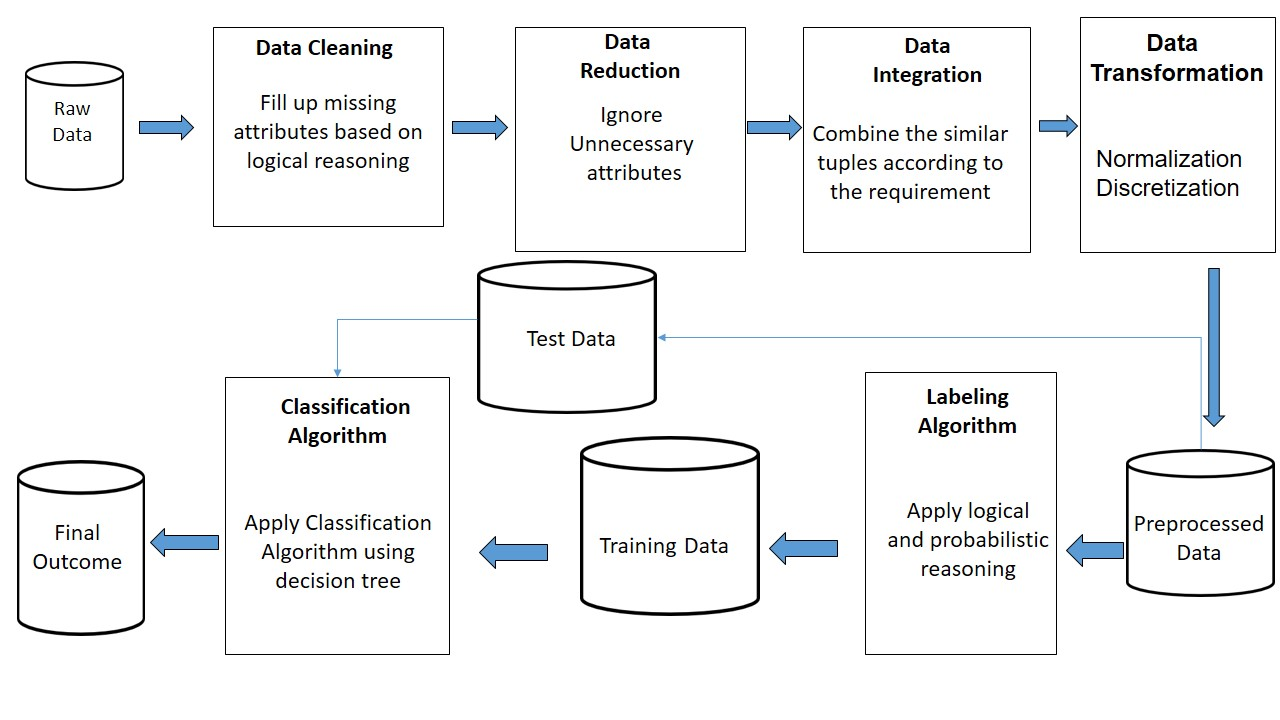
\includegraphics[width=\linewidth]{Figures/classification.jpg}
  \decoRule
  \caption[Classification]{General Process of Classification}
  \label{fig:classification}
\end{figure}

Figure ~\ref{fig:classification} shows the general procedure of classification.
\subsection{Decision Tree Induction}
\paragraph{}
Decision tree induction is the learning of decision trees from class-labeled training tuples. A decision tree is a
flowchart-like tree structure, where each internal node (nonleaf node) denotes a test on an attribute, each
branch represents an outcome of the test, and each leaf node (or terminal node) holds a class label. The
topmost node in a tree is the root node. 
The decision tree in Figure ~\ref{fig:decisiontree} is a tree for the concept buy\_computer that indicates whether a customer at a company is likely to buy a computer or not. Each internal node represents a test on an attribute. Each leaf node represents a class.
The benefits of having a decision tree are 
\begin{itemize}
\item It does not require any domain knowledge.
\item is easy to comprehend.
\item The learning and classification steps of a decision tree are simple and fast.
\end{itemize}
    

\begin{figure}
   \centering
  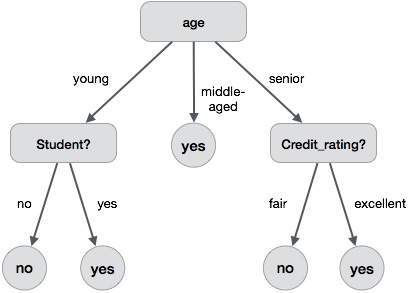
\includegraphics[width=\linewidth]{Figures/dm_decision_tree.jpg}
  \decoRule
  \caption[A Decision Tree]{A Decision Tree}
  \label{fig:decisiontree}
\end{figure}

\subsection{Decision Tree Induction Algorithm}
A machine researcher named J. Ross Quinlan in 1980 developed a decision tree algorithm known as ID3 (Iterative Dichotomiser). Later, he presented C4.5, which was the successor of ID3. ID3 and C4.5 adopt a greedy approach. In this algorithm, there is no backtracking; the trees are constructed in a top-down recursive divide-and-conquer manner.

{\SetAlgoNoLine
\begin{algorithm}[H]

\label{generatedecisiontree}
\SetKwInOut{Input}{Input}
\SetKwInOut{Output}{Output}

\Input{ \begin{itemize}
\item Data partition, D, which is a set of training tuples and their associated class labels;
\item $attribute\_list$, the set of candidate attributes\;
\item $Attribute\_selection\_method $.
\end{itemize}}
\Output{A decision tree.}

\begin{algorithmic}[1]
\caption{Generate\_decision\_tree}
\Procedure{}{}
    \State create a node $N$\;
    \If{tuples in $D$ are all of the same class, $C$,}{
    	return $N$ as leaf node labeled with the class $C$ \;
    }
    
    \If{$attribute\_list$ is empty}{
    	return $N$ as leaf node labeled with the majority class in $D$ \;
    }
   \State apply $Attribute\_selecction\_method(D,attribute\_list)$ to find best splitting\-criterion \;  
        
   \State label node $N$ with $splitting_criterion$ \;
    \If{$splitting\_criterion$ is discrete valued and multiway splits allowed}
   {$ attribute\_list \leftarrow attribute\_list - splitting\_ttribute $\;
   } 
      \For {each outcome $j$ of $splitting\_criterion$}{
        \State let $D_j$ be the set of data tuples in $D$ satisfying outcome $j$ \; 
        \If{$D_j is empty$}
        {
        	attach a leaf labeled with the majority class in $D$ to node $N$ \;
        }
        \Else {attach a leaf labeled with the majority class in $D$ to node $N$ \;}
	}
\State return $N$ \;
\EndProcedure
\end{algorithmic}
\end{algorithm}}

Algorithm ~\ref{generatedecisiontree} is the general approach to build a decision tree.

\subsection{Attributes Selection Measures}
\paragraph{}
An attribute selection measure is a heuristic for selecting the splitting criterion that "best" separates a given
data partition, D, of class-labeled training tuples into individual classes. If we were to split D into smaller
partitions according to the outcomes of the splitting criterion, ideally each partition would be pure (i.e., all the
tuples that fall into a given partition would belong to the same class). Conceptually, the "best" splitting
criterion is the one that most closely results in such a scenario. Attribute selection measures are also known as
splitting rules because they determine how the tuples at a given node are to be split. \newline
The attribute selection measure provides a ranking for each attribute describing the given training tuples. The
attribute having the best score for the measure\footnote{\label{third}Depending on the measure, either the highest or lowest score is chosen as the best (i.e., some measures strive to maximize while others strive to minimize).} is chosen as the splitting attribute for the given tuples. If the
splitting attribute is continuous-valued or if we are restricted to binary trees, then, respectively, either a split
point or a splitting subset must also be determined as part of the splitting criterion. The tree node created for
partition D is labeled with the splitting criterion, branches are grown for each outcome of the criterion, and the
tuples are partitioned accordingly.Three popular attribute selection measures are

\begin{itemize}
\item Information gain
\item Gain ration
\item Gini index
\end{itemize}
The notation used herein is as follows. Let $D$, the data partition, be a training set of class labeled tuples.
Suppose the class label attribute has m distinct values defining m distinct classes, $C_i$ (for $i=1,2,....$). Let
be the set of tuples of class $C_i$ in $D$. Let $|D|$ and $|C_{i,D}|$ denote the number of tuples in $D$ and $C_{i,D}$
respectively.
\subsubsection{Information Gain}\label{infogain}
\paragraph{}
ID3 uses information gain as its attribute selection measure. This measure is based on pioneering work by
Claude Shannon on information theory, which studied the value or "information content" of messages. Let
node N represent or hold the tuples of partition D. The attribute with the highest information gain is chosen as
the splitting attribute for node N. This attribute minimizes the information needed to classify the tuples in the
resulting partitions and reflects the least randomness or "impurity" in these partitions. Such an approach
minimizes the expected number of tests needed to classify a given tuple and guarantees that a simple (but not
necessarily the simplest) tree is found.
\paragraph{}
The expected information needed to classify a tuple in D is given by $$ Info(D)= -\sum(p_i*\log(p_i)) $$
where $p_i$ is the nonzero probability that an arbitrary tuple in $D$ belongs to class $C_i$ and is estimated by $|C_{i,D}|/|D|$. A log function to the base 2 is used, because the information is encoded in bits. $Info(D)$ is just the average amount of information needed to identify the class label of a tuple in $D$. Note that, at this point, the
information we have is based solely on the proportions of tuples of each class. $Info(D)$ is also known as the
entropy of $D$.
How much more information would we still need (after the partitioning) to arrive at an exact classification?
This amount is measured by $$Info_A(D)=\sum{\dfrac{|D_j|}{|D|}*Info(D_j)} $$
nformation gain is defined as the difference between the original information requirement (i.e., based on just
the proportion of classes) and the new requirement (i.e., obtained after partitioning on A). That is,
$$Gain(A)=Info(D)-Info_A(D)$$

\subsubsection{Gain Ratio}
\paragraph{}
The information gain measure is biased toward tests with many outcomes. That is, it prefers to select attributes
having a large number of values. For example, consider an attribute that acts as a unique identifier such as
$product\_ID$. A split on $product\_ID$ would result in a large number of partitions (as many as there are values),
each one containing just one tuple. Because each partition is pure, the information required to classify data set
D based on this partitioning would be $Info_product\_ID(D)=0$ . Therefore, the information gained by partitioning on this attribute is maximal. Clearly, such a partitioning is useless for classification.
\paragraph{}
C4.5, a successor of ID3, uses an extension to information gain known as gain ratio, which attempts to
overcome this bias. It applies a kind of normalization to information gain using a "split information" value
defined analogously with $Info(D)$ as $$SplitInfo_A(D)=-\sum(\dfrac{|D_j|}{|D|}* \log_2(\dfrac{|D_j|}{|D|}))$$
This value represents the potential information generated by splitting the training data set, $D$, into $v$ partitions,
corresponding to the v outcomes of a test on attribute A. Note that, for each outcome, it considers the number of
tuples having that outcome with respect to the total number of tuples in D. It differs from information gain,
which measures the information with respect to classification that is acquired based on the same partitioning.
The gain ratio is defined as $$GainRatio=\dfrac{Gain(A)}{SplitInfo_A(D)} $$

\subsubsection{Gini Index}

The Gini index is used in CART. Using the notation previously described, the Gini index measures the impurity
of D, a data partition or set of training tuples, as $$Gini(D)=1-\sum(p_i^{2}) $$

where pi is the probability that a tuple in $D$ belongs to class $C_i$ and is estimated by $|C_{i,D}|/|D|$ . The sum is computed over $m$ classes.

When considering a binary split, we compute a weighted sum of the impurity of each resulting partition. For
example, if a binary split on A partitions $D$ into $D_1$ and $D_2$, the Gini index of D given that partitioning is
$$Gini_A(D)=\dfrac{|D_1|}{|D|}Gini(D_1) +  \dfrac{|D_2|}{|D|}Gini(D_2).$$

The reduction in impurity that would be incurred by a binary split on a discrete- or continuous-valued attribute
A is $$\delta{}Gini(A)=Gini(D)-Gini_A(D).$$

\subsubsection{Other Attribute Selection Measures}

Many other attribute selection measures have been proposed. CHAID, a decision tree algorithm that is popular
in marketing, uses an attribute selection measure that is based on the statistical $\chi^{2} $ test for independence. Other measures include C-SEP (which performs better than information gain and the Gini index in certain cases) and
G-statistic (an information theoretic measure that is a close approximation to $\chi^{2} $ distribution).\\
Attribute selection measures based on the Minimum Description Length (MDL) principle have the least bias
toward multivalued attributes. MDL-based measures use encoding techniques to define the "best”" decision tree
as the one that requires the fewest number of bits to both (1) encode the tree and (2) encode the exceptions to
the tree(i.e., cases that are not correctly classified by the tree). Its main idea is that the simplest of solutions is preferred. \\
Other attribute selection measures consider multivariate splits (i.e., where the partitioning of tuples is based
on a combination of attributes, rather than on a single attribute). The CART system, for example, can find
multivariate splits based on a linear combination of attributes. Multivariate splits are a form of attribute (or
feature) construction, where new attributes are created based on the existing ones.

 
% Chapter 1

\chapter{Analysis of BIIS Data} % Main chapter title

\label{Analysis of BIIS Data} % For referencing the chapter elsewhere, use \ref{Chapter1} 

%----------------------------------------------------------------------------------------

% Define some commands to keep the formatting separated from the content 

%----------------------------------------------------------------------------------------
\section{Scope}
BUET offers educational facilities for more than 5000 students in an academic session.
These students are under  departments.Number of students in a respective department is different according to the department facility.Department of Electrical \& Electronic Engineering, Department of Civil Engineering, Department of Mechanical Engineering can afford 195 students per batch. Department of Computer Science \& Engineering has 120 students. Department of Architecture afford 55 students,Department of Water Resource Engineering,Department of Materials \& Metallurgical Engineering,Department of Urban \& Regional Planning and Department of Industrial \& Production Engineering hold 30 students each. Department of Naval Architecture \& Marine Engineering and Department of Chemical Engineering has 60 students each \cite{buet}. These numbers have been changed throughout year by year but 
it represent the period on which this research has been more focused.
In this research BIIS data of 10 already graduated batches have been used which represents almost 10 thousand students.Academic performance of no current student has been brought under this research. 

%----------------------------------------------------------------------------------------

\section{Database Structure}
There are 8 parts of BIIS data and each data sheet has 65,000 tuples.Each tuple represents the performance of a student in a particular course.The attributes of the tuple are described below
\begin{itemize}
\item Serial : It is the serial number of a particular student.It is not actually the student id,but it's a unique constraint and primary key of the database table.
\item Department : Respective department of the student.
\item HallStatus : Indicates whether the student is hall resident or attached.
\item District : Home district of the student.
\item Thana : Thana of the student.
\item Gender : Gender of the student.
\item PlaceOfBirth : Birth place of the student.
\item StartingOfAcademicYear : Indicates on which academic year the student has started undergrad.
\item AdmissionDate : Admission day at BUET.
\item CourseName : The particular course taken by student.
\item LetterGrade : Lettergrade of the respective course. 
\item ClassAttendanceMark : It represents the attendance mark of the student in respective course.The attendance mark is allocated 10\% of total course mark.E.g.,For 3 credit courses,it's marked out of 30,for 4 credit course it's marked out of 40. 
\item ClassTestMark : Class test mark is allocated 20\% of the total number of a course.E.g.,For 3 credit course,highest ct mark is 60,for 4 credit course it's 80.
\item PartAMark :  For theory courses the term final examination holds 70\% weight of total course.This huge exam is divided into 2 parts. Generally internal examiner handles Part A.E.g., For 3 credit course,part A holds 105 marks,for 4 credit courses it's 140.
\item PartBMark : Same as part A,generally external examiner handles part B.
\item TotalNumber : Total mark obtained by a student in a particular course..
\item LevelName : The level respective course has been taken.
\item TermName : The term respective course has been taken.
\item GPA : GPA of student in particular term.
\item CGPA : CGPA upto the respective term.
\item TermCount : Term count of the student.
\item CreditHourEarned : Credit hour earned by the student in the respective term.
\item TotalCreditHourCompleted : Total credit hour earned by the student upto respective term.
\end{itemize}



\section{Problems in Existing Structure}
The universal database holds raw academic data of the students.There are plenty of disturbance in this database.They are described below :
\begin{itemize}
\item The first and most important problem is, all the eight data sheets don't have same attributes among them.For example, Sheet 1 doesn't have a \textit{CourseName} column whereas Sheet 2 has one.There are many more incidents where attributes don't match.
\item One student enrolls into a number of courses in academic career which can vary from 65 to 80.So, there are multiple tuple for one student which is not suitable for classification.Determining status from multiple tuples is very difficult. Table \ref{tab:t1} is an example of this.
\begin {table}[H]
\caption {Multiple entries for single student in the Universal Database} \label{tab:t1} 
\begin{center}
\begin{tabular}{ | m{2cm} | m{2cm}| m{0.5cm} | m{3cm} | m{2cm} | m{0.5cm} | } 
\hline
Serial & Department & ... & CourseName & LetterGrade & ... \\ 
\hline
2 & CE & ... & PHY143 & A- & ... \\ 
\hline
2 & CE & ... & MATH141 & B+ & ... \\ 
\hline
... & ... & ... & ... & ... & ... \\ 
\hline
\end{tabular}
\end{center}
\end{table}
\item The database is in a format of full outer join.So, there are plenty of blank attributes.For example, in sessional courses,there is no Part A or Part B. So, \textit{PartAMark} or \textit{PartBMark} remains void for sessional courses. Besides, there are also some special course for which maximum attributes remain blank. 
\begin {table}[H]
\caption {Blank attributes in Database} \label{tab:title} 
\begin{center}
\begin{tabular}{ | m{1cm} | m{2cm}| m{0.5cm}| m{2cm} | m{2cm} | m{2cm} |  m{0.5cm} | } 
\hline
Serial & Department & ... & CourseName & PartAMark & PartBMark & ... \\ 
\hline
65 & CSE & ... & CSE100 & - & - & ... \\ 
\hline
65 & CSE & ... & MATH141 & 93 & 112 & ... \\ 
\hline
... & ... & ... & ... & ... & ... & ... \\ 
\hline
\end{tabular}
\end{center}
\end{table}
\item There are some attributes,for which there is no value was really inserted ever.In some datasheets \textit{PlaceOfBirth,District,Thana} are blank.
\item In some data sheets, \textit{CGPA \& GPA} have rounded value. But, for accurate results, it is very important to get the accurate \textit{CGPA \& GPA} upto two floating points at least.
\begin {table}[H]
\caption {Rounded up value of CGPA and GPA} \label{tab:title} 
\begin{center}
\begin{tabular}{ | m{1cm} |  m{2cm} | m{0.5cm}| m{2cm} | m{2cm} | m{0.5cm} | } 
\hline
Serial & Department & ... & GPA & CGPA  & ... \\ 
\hline
4478 & NAME & ... & 4 & 3 & ... \\ 
\hline
4478 & NAME & ... & 3 & 3 & ... \\ 
\hline
... & ... & ... & ... & ... & ... \\ 
\hline
\end{tabular}
\end{center}
\end{table}
\item There is no \textit{CourseCredit} attribute in the database.But for proper reasoning,\textit{CourseCredit} is very important.
\item Some attributes like \textit{TotalCreditHourCompleted,AttendanceMarks,ClassTestMark} don't have the same range of value for all the tuples.So, any reasoning from these values is very difficult.
\begin {table}[H]
\caption {Different range of values} \label{tab:title} 
\begin{center}
\begin{tabular}{ | m{1cm} | m{2cm}| m{0.5cm}| m{2cm} | m{2cm} | m{2cm} |  m{0.5cm} | } 
\hline
Serial & Department & ... & Attendance\newline Mark & ClassTest\newline Mark & Total\newline CreditHour\newline Completed & ... \\ 
\hline
65 & CSE & ... & 27 & 44 & 160 & ... \\ 
\hline
120 & ARCH & ... & 40 & 71 & 190 & ... \\ 
\hline
... & ... & ... & ... & ... & ... & ... \\ 
\hline
\end{tabular}
\end{center}
\end{table}
\item There are many confusing attributes like \textit{TermCount,AdmissionDate} which don't actually make sense.
\item Reasoning for Theory and Sessional courses are entirely different,but this database don't indicate whether a course is Theory course or not.

\end{itemize}
% Chapter 4

\chapter{Preprocessing} % Main chapter title

\label{Preprocessing} % For referencing the chapter elsewhere, use \ref{Chapter1} 

%----------------------------------------------------------------------------------------

% Define some commands to keep the formatting separated from the content 

%----------------------------------------------------------------------------------------

\section{Technique And Design}

%----------------------------------------------------------------------------------------

\section{Algorithms}
\subsection{Cleaning}
\subsection{Reduction}
\subsection{Integration}
\subsection{Normalization}

%----------------------------------------------------------------------------------------

\section{Results}

 
% Chapter 5

\chapter{Classification} % Main chapter title

\label{Classification} % For referencing the chapter elsewhere, use \ref{Chapter1} 
There are five class labels in our classification model.They are
\begin{itemize}
\item Excellent
\item Good
\item Moderate
\item Poor
\item Very Poor
\end{itemize}
Applying ID3 classification algorithm a decision tree was created using training data and this knowledge in decision tree was used to find the class label of test data set.
%----------------------------------------------------------------------------------------

% Define some commands to keep the formatting separated from the content 

%----------------------------------------------------------------------------------------

\section{Decision Tree}
The training data was prepared after data preprocessing as described in Chaper \ref{Preprocessing}.The final attributes in the training data are
\begin{itemize}
\item Student Id 
\item Department	
\item Hall Status 	
\item Gender 	
\item Attendance marks 	
\item Class test marks 	
\item Earned CGPA 
\item Completed Credit 
\item Final status according to our reasoning as Status
\end{itemize}
A sample of the training data set looks like Table \ref{tab:Training Data}.


\begin{table}
\caption{Training Data Sample}
\label{tab:Training Data}
\centering
\begin{tabular}{l l l l l l l l l}
\toprule
\tabhead{SID} & \tabhead{Department} & \tabhead{Hall}& \tabhead{Gender}& \tabhead{Attendance}& \tabhead{ClassTest} & \tabhead{Cgpa}& \tabhead{Credit}& \tabhead{Status}\\
\midrule
4650  & 2& 0 &1	& 1 &	0.83 & 	3.72 & 1 &	excellent\\
4755 & 9 & 1 & 1 & 0.82	& 0.71 &	3.39 &	1 &	poor \\
4769 &	1 &	1 &	1 &	0.97 &	0.83 &	3.76 & 	0.98 &	moderate\\
4975 &	3 & 1 & 0 & 0.99 &	0.76 & 	3.50 &	1 &	good \\
5064 &	10 & 0 &  1 & 	0.33 & 	0.33 &	2.61 & 	0.75 & very poor \\

\bottomrule\\
\end{tabular}
\end{table}

%----------------------------------------------------------------------------------------
A hypothetical decision tree can be derived from the training data as depicted in Figure \ref{fig:Decision Tree From BIIS Training Data}. 

\begin{figure}
   \centering
  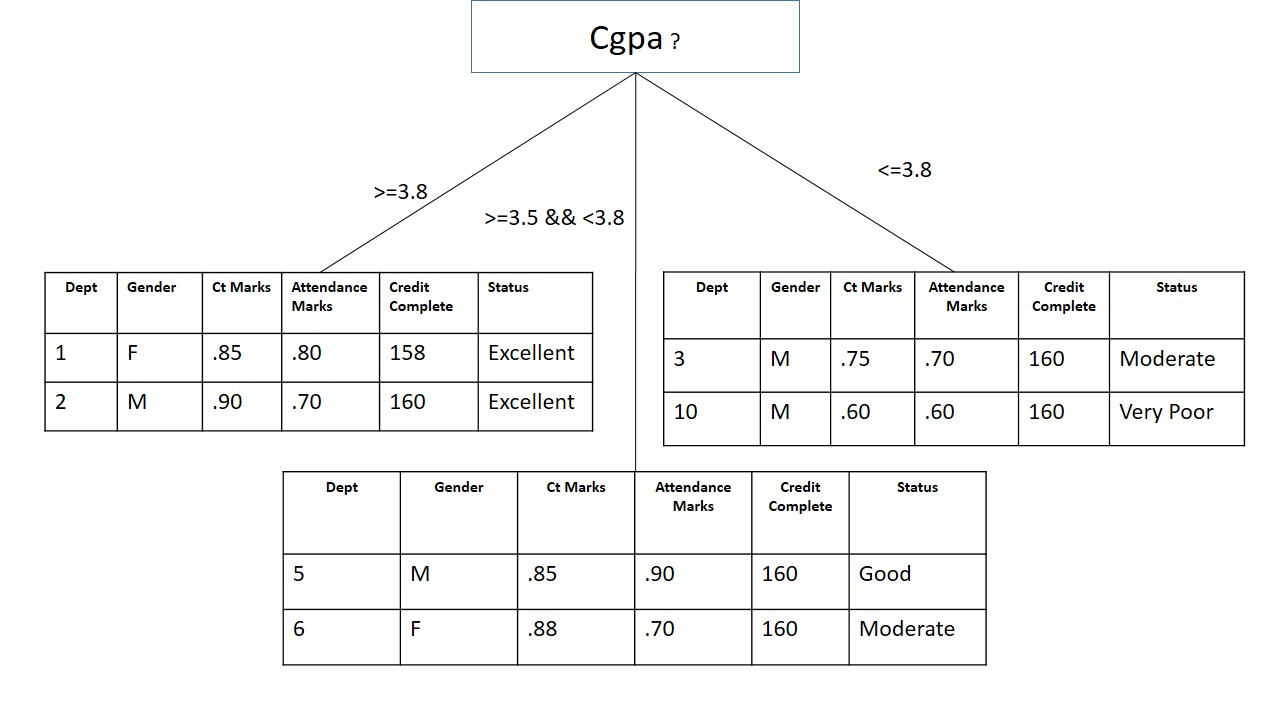
\includegraphics[width=\linewidth]{Figures/Presentation1_2.jpg}
  \decoRule
  \caption[A Decision Tree From Training Data]{A Decision Tree From Training Data}
  \label{fig:Decision Tree From BIIS Training Data}
\end{figure}

\section{Algorithm}
The algorithm used is ID3 Algorithm. So, Information gain as described in Section \ref{infogain} is used as splitting criterion. \\
We used the structure of the algorithm described in Algorithm \ref{generatedecisiontree} in our implementation. We used Java programming language for implementation. \\
The pseudocode for the final implementation of the algorithm is shown 



\begin{algorithm}[H]

\label{generatedecisiontreeforbiisdata}
\SetKwInOut{Input}{Input}
\SetKwInOut{Output}{Output}

\Input{ \begin{itemize}
\item Data partition, D, which is a set of training tuples and their associated class labels;
\item $attribute\_list(SID,Department,Hall,Attendance,ClassTest,Cgpa,CreditComplete)$, the set of candidate attributes\;
\item $Attribute\_selection\_method : Information gain with majority voting$.
\end{itemize}}
\Output{A decision tree.}

\begin{algorithmic}[1]
\caption{Generate\_decision\_tree\_For\_BIIS\_Data}
\Procedure{}{}
    \State create a node $N$\;
    \If{tuples in $D$ are all of the same class, $C$,}{
    	return $N$ as leaf node labeled with the class $C$ \;
    }
    
    \If{$attribute\_list$ is empty}{
    	return $N$ as leaf node labeled with the majority class in $D$ \;
    }
   \State apply $Attribute\_selecction\_method(D,attribute\_list)$ to find best splitting\-criterion \;  
        
   \State label node $N$ with $splitting_criterion$ \;
    \If{$splitting\_criterion$ is Dept or Hall\_Status or Gender}
   {
   \State split according to the discrete values of the attribure\;\\
   $ attribute\_list \leftarrow attribute\_list - splitting\_attribute $\;
   } 
  
   \Else
   {
   		\Comment $splitting\_criterion$ is Cgpa or Attendance or Classtest or CreditCompleted. \\
   		\State split 3 ways according to the values of the attribute for example for Cgpa divide at 3.8 and 3.5 into 			3 parts\;\\
   		$ attribute\_list \leftarrow attribute\_list - splitting\_attribute $\;
   } 
      
      \For {each outcome $j$ of $splitting\_criterion$}{
        \State let $D_j$ be the set of data tuples in $D$ satisfying outcome $j$ \; 
        \If{$D_j is empty$}
        {
        	attach a leaf labeled with the majority class in $D$ to node $N$ \;
        }
        \Else {attach a leaf labeled with the majority class in $D$ to node $N$ \;}
	}
\State return $N$ \;
\EndProcedure
\end{algorithmic}
\end{algorithm}

\section{Result of Classification}
 
\begin{table}
\caption{Training Data Sample}
\label{tab:Test Data Sample}
\centering
\begin{tabular}{|c| c| c| c| c| c|c | c|c }
\toprule
\tabhead{SID} & \tabhead{Department} & \tabhead{Hall}& \tabhead{Gender}& \tabhead{Attendance}& \tabhead{ClassTest} & \tabhead{Cgpa}& \tabhead{Credit} \\
\midrule
4487	&9&	1&	1	&0.98&	0.77&	3.64&	1\\
4488	&9&	0&	0&	0.72&	0.68&	3.18&	1\\
4489	&9	&0&	0&	0.93&	0.69&	3.49&	1\\
4490	&9	&1	&1	&0.61&	0.59&	3.02&	0.96\\
4492	&11	&1	&1	&0.99&	0.72&	3.06&	0.99\\
4493	&11&	1&	1&	0.71&	0.68&	3.07&	0.91\\
4488	&9	&0	&0	&0.72	&0.68	&3.18&	1\\
4489	&9	&0	&0	&0.93	&0.69	&3.49&	1\\
4490	&9	&1	&1	&0.61	&0.59	&3.02&	0.96\\
4492	&11	&1	&1	&0.99	&0.72	&3.06&	0.99\\
4493	&11	&1	&1	&0.71	&0.68	&3.07&	0.91\\
4494	&11	&1	&0	&0.89	&0.78	&3.25&	0.99\\
4496	&11	&0	&1	&0.98	&0.73	&3.22&	0.99\\


\bottomrule
\end{tabular}
\end{table}


Test data set before applying algorithm looks like Table ~\ref{tab:Test Data Sample}.

\begin{table}
\caption{Final Output Sample}
\label{tab:Final Result}
\centering
\begin{tabular}{|c| c| c| c| c| c|c | c|c|c }
\toprule
\tabhead{SID} & \tabhead{Department} & \tabhead{Hall}& \tabhead{Gender}& \tabhead{Attendance}& \tabhead{ClassTest} & \tabhead{Cgpa}& \tabhead{Credit} & \tabhead{Status} \\
\midrule
4487	& 9 &	1 &	1	& 0.98 &	0.7 7&	3.64 &	1 & good\\
4488	& 9 &	0 &	0 &	0.72 &	0.68 &	3.18 &	1 & moderate\\
4489	& 9	& 0 &	0 &	0.93 &	0.69 &	3.49 &	1 & good\\
4490	& 9	& 1	& 1	& 0.61 &	0.59 &	3.02 &	0.96 & poor\\
4492	& 11	& 1	& 1	& 0.99 &	0.72 &	3.06 &	0.99 & moderate\\
4493	& 11 &	1 &	1 &	0.71 &	0.68 &	3.07 &	0.91 & poor\\
4488	& 9	& 0	& 0	& 0.72	& 0.68	& 3.18 &	1 & moderate\\
4489	& 9	& 0	& 0	& 0.93	& 0.69	& 3.49 &	1 & good\\
4490	& 9	& 1	& 1	& 0.61	& 0.59	& 3.02 &	0.96 & very poor\\
4492	& 11	& 1	& 1	& 0.99	& 0.72	& 3.06 &	0.99 & poor\\
4493	& 11	& 1	& 1	& 0.71	& 0.68	& 3.07 &	0.91 & very poor\\
4494	& 11	& 1	& 0	& 0.89	& 0.78	& 3.25 &	0.99 & moderate\\
4496	& 11	& 0	& 1	& 0.98	& 0.73	& 3.22 &	0.99 & moderate\\


\bottomrule
\end{tabular}
\end{table}

After applying algortihm as desribed in Algorithm \ref{generatedecisiontreeforbiisdata} the results as shown in Table \ref{tab:Final Result} are found.

%----------------------------------------------------------------------------------------

\section{Statistical Analysis}

We analyzed the final results and found some relevant statistical results. The categories are\:
\begin{itemize}
\item Department wise performance
\item Impact of gender on performance
\item Impact of hall status on performance
\item Impact of classtest marks on performance
\item Impact of attendance marks on performance
\item Impact of cgpa on performance
\item Impact of credit completion on performance
\end{itemize}
The details of the findings are discussed in Section \ref{resultofanlysis}
%----------------------------------------------------------------------------------------

\section{Result of Statistical Analysis}\label{resultofanlysis}

\subsection{Department wise Performance}
\subsubsection{EEE Department}
The overall performance of EEE department is shown in Figure \ref{fig:Performance of EEE Department}.
\begin{table}
\caption{Performance of EEE department}
\label{tab:eee}
\centering
\begin{tabular}{|c| c| }
\toprule
\tabhead{Class Label} & \tabhead{Percent}\\
\midrule
Excellent & $18\%$\\
Good & $42\%$\\
Moderate & $32\%$\\
Poor & $5\%$\\
Very Poor & $3\%$\\

\bottomrule
\end{tabular}
\end{table}
According to our classifier the percentage of each class label of EEE department is shown in Table \ref{tab:eee}

\begin{figure}
   \centering
  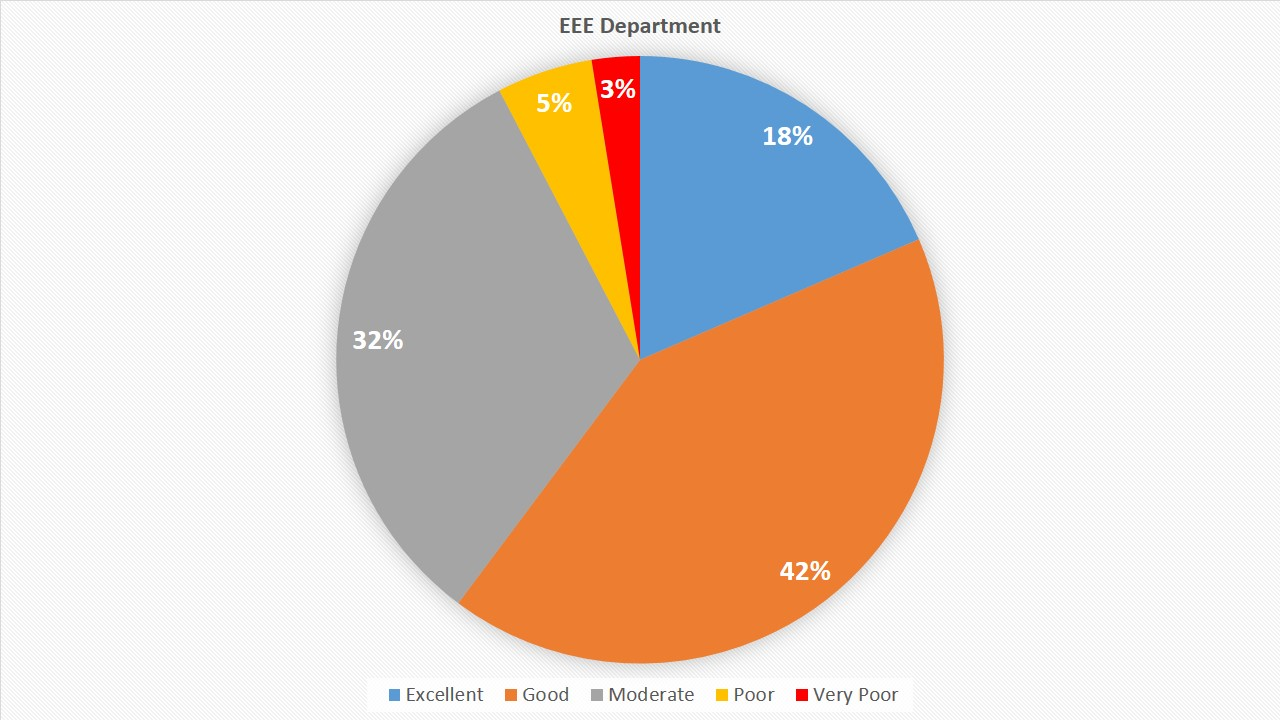
\includegraphics[width=\linewidth]{Figures/Slide3.jpg}
  \decoRule
  \caption[Performance of EEE Department]{Performance of EEE Department}
  \label{fig:Performance of EEE Department}
\end{figure}


\subsubsection{CSE Department}
The overall performance of CSE department is shown in Figure \ref{fig:Performance of CSE Department}.
\begin{table}
\caption{Performance of CSE Department}
\label{tab:cse}
\centering
\begin{tabular}{|c| c| }
\toprule
\tabhead{Class Label} & \tabhead{Percent}\\
\midrule
Excellent & $21\%$\\
Good & $32\%$\\
Moderate & $12\%$\\
Poor & $30\%$\\
Very Poor & $5\%$\\
\bottomrule
\end{tabular}
\end{table}
According to our classifier the percentage of each class label of CSE department is shown in Table \ref{tab:cse}

\begin{figure}
   \centering
  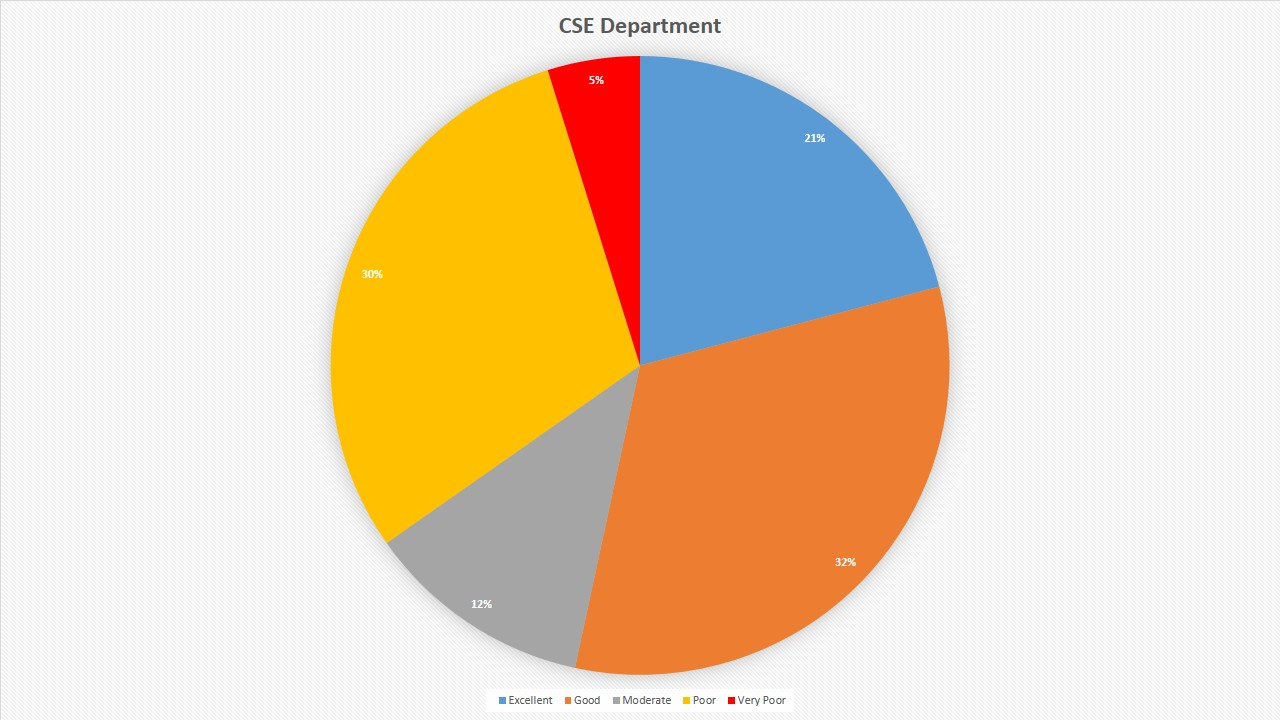
\includegraphics[width=\linewidth]{Figures/Slide2.jpg}
  \decoRule
  \caption[Performance of CSE Department]{Performance of CSE Department}
  \label{fig:Performance of CSE Department}
\end{figure}



\subsubsection{IPE Department}
The overall performance of IPE department is shown in Figure \ref{fig:Performance of IPE Department}.
\begin{table}
\caption{Performance of IPE Department}
\label{tab:ipe}
\centering
\begin{tabular}{|c| c| }
\toprule
\tabhead{Class Label} & \tabhead{Percent}\\
\midrule
Excellent & $13\%$\\
Good & $33\%$\\
Moderate & $17\%$\\
Poor & $23\%$\\
Very Poor & $14\%$\\

\bottomrule
\end{tabular}
\end{table}
According to our classifier the percentage of each class label of IPE department is shown in Table \ref{tab:ipe}

\begin{figure}
   \centering
  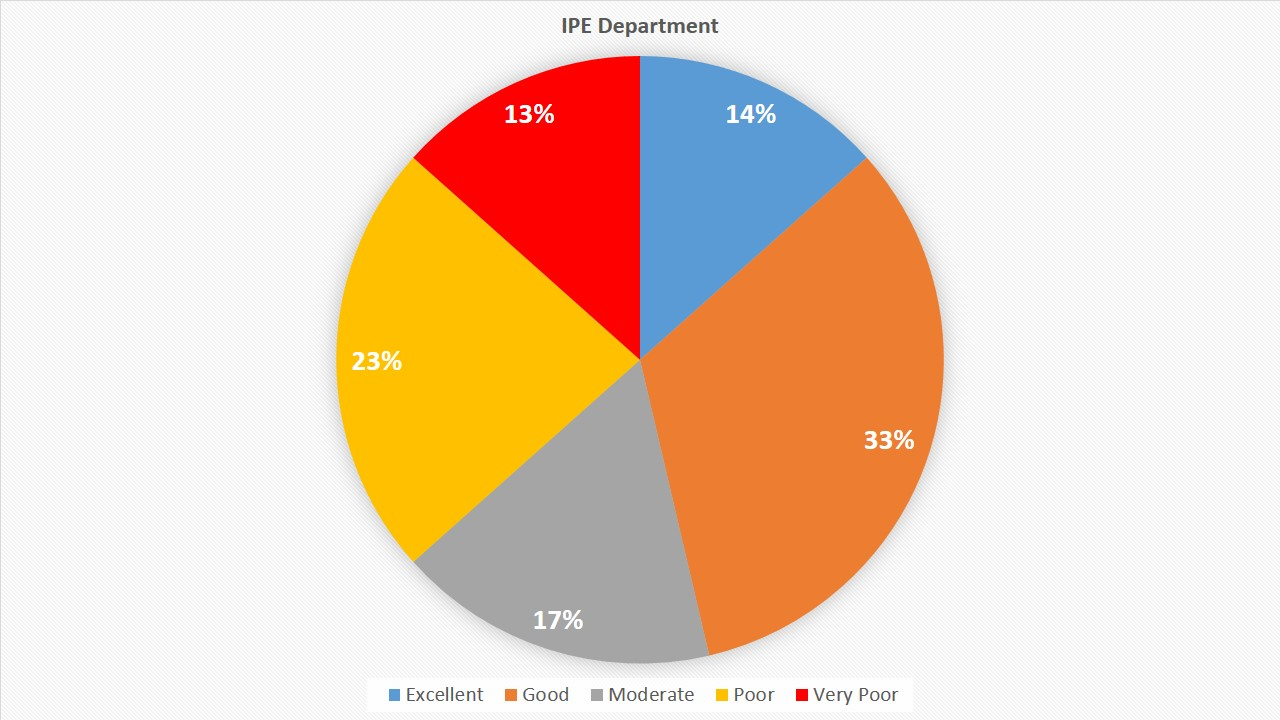
\includegraphics[width=\linewidth]{Figures/Slide4.jpg}
  \decoRule
  \caption[Performance of IPE Department]{Performance of IPE Department}
  \label{fig:Performance of IPE Department}
\end{figure}





\subsubsection{ME Department}
The overall performance of ME department is shown in Figure \ref{fig:Performance of ME Department}.
\begin{table}
\caption{Performance of ME Department}
\label{tab:me}
\centering
\begin{tabular}{|c| c| }
\toprule
\tabhead{Class Label} & \tabhead{Percent}\\
\midrule
Excellent & $5\%$\\
Good & $42\%$\\
Moderate & $37\%$\\
Poor & $6\%$\\
Very Poor & $10\%$\\

\bottomrule
\end{tabular}
\end{table}
According to our classifier the percentage of each class label of ME department is shown in Table \ref{tab:me}

\begin{figure}
   \centering
  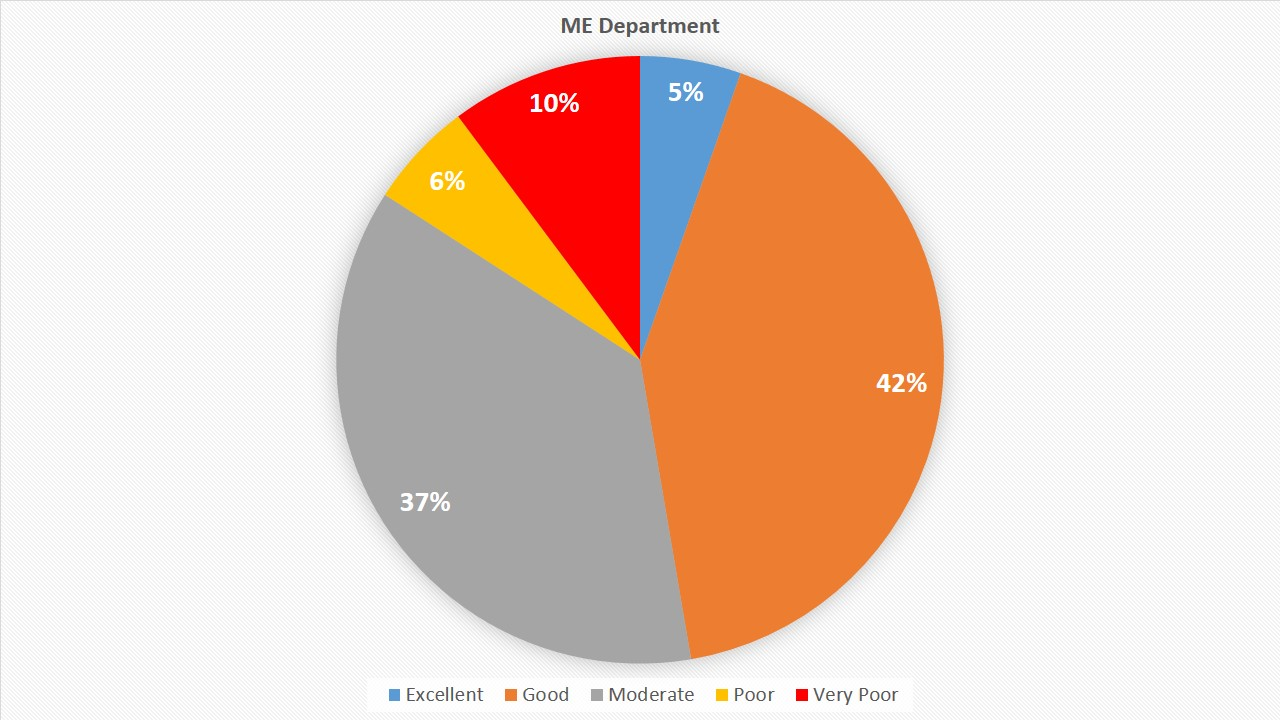
\includegraphics[width=\linewidth]{Figures/Slide5.jpg}
  \decoRule
  \caption[Performance of ME Department]{Performance of ME Department}
  \label{fig:Performance of ME Department}
\end{figure}




\subsubsection{CE Department}
The overall performance of CE department is shown in Figure \ref{fig:Performance of CE Department}.
\begin{table}
\caption{Performance of CE Department}
\label{tab:ce}
\centering
\begin{tabular}{|c| c| }
\toprule
\tabhead{Class Label} & \tabhead{Percent}\\
\midrule
Excellent & $5\%$\\
Good & $27\%$\\
Moderate & $47\%$\\
Poor & $15\%$\\
Very Poor & $6\%$\\

\bottomrule
\end{tabular}
\end{table}
According to our classifier the percentage of each class label of CE department is shown in Table \ref{tab:ce}

\begin{figure}
   \centering
  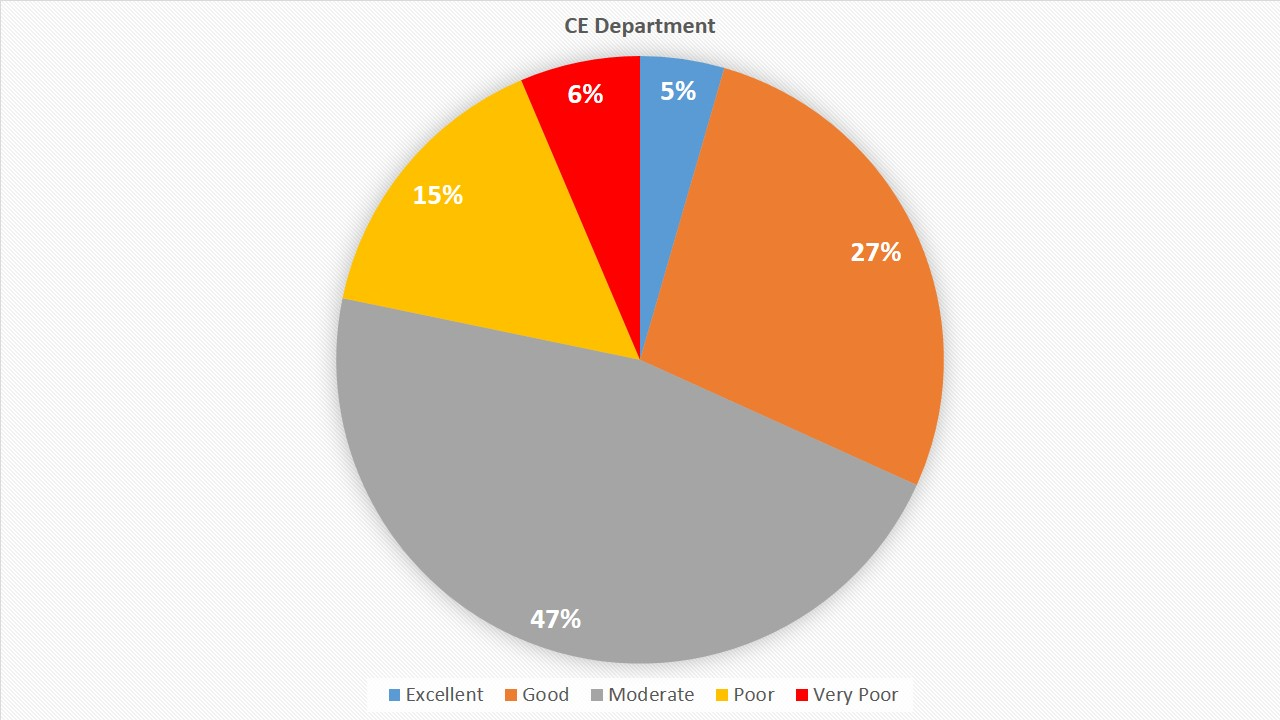
\includegraphics[width=\linewidth]{Figures/Slide6.jpg}
  \decoRule
  \caption[Performance of CE Department]{Performance of CE Department}
  \label{fig:Performance of CE Department}
\end{figure}





\subsubsection{MME Department}
The overall performance of MME department is shown in Figure \ref{fig:Performance of MME Department}.
\begin{table}
\caption{Performance of MME Department}
\label{tab:mme}
\centering
\begin{tabular}{|c| c| }
\toprule
\tabhead{Class Label} & \tabhead{Percent}\\
\midrule
Excellent & $16\%$\\
Good & $37\%$\\
Moderate & $22\%$\\
Poor & $14\%$\\
Very Poor & $11\%$\\
\bottomrule
\end{tabular}
\end{table}
According to our classifier the percentage of each class label of MME department is shown in Table \ref{tab:mme}

\begin{figure}
   \centering
  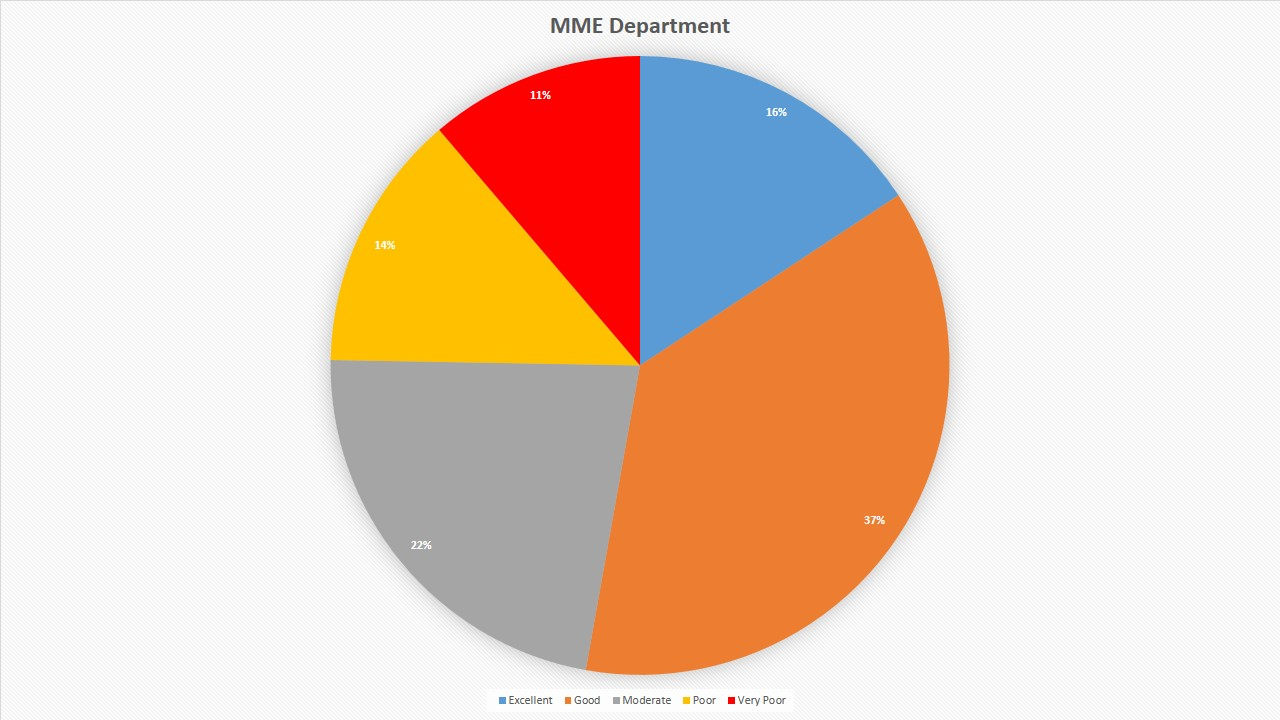
\includegraphics[width=\linewidth]{Figures/Slide7.jpg}
  \decoRule
  \caption[Performance of MME Department]{Performance of MME Department}
  \label{fig:Performance of MME Department}
\end{figure}



\subsubsection{CHE Department}
The overall performance of CHE department is shown in Figure \ref{fig:Performance of CHE Department}.
\begin{table}
\caption{Performance of CHE Department}
\label{tab:che}
\centering
\begin{tabular}{|c| c| }
\toprule
\tabhead{Class Label} & \tabhead{Percent}\\
\midrule
Excellent & $5\%$\\
Good & $62\%$\\
Moderate & $13\%$\\
Poor & $8\%$\\
Very Poor & $12\%$\\

\bottomrule
\end{tabular}
\end{table}
According to our classifier the percentage of each class label of CHE department is shown in Table \ref{tab:che}

\begin{figure}
   \centering
  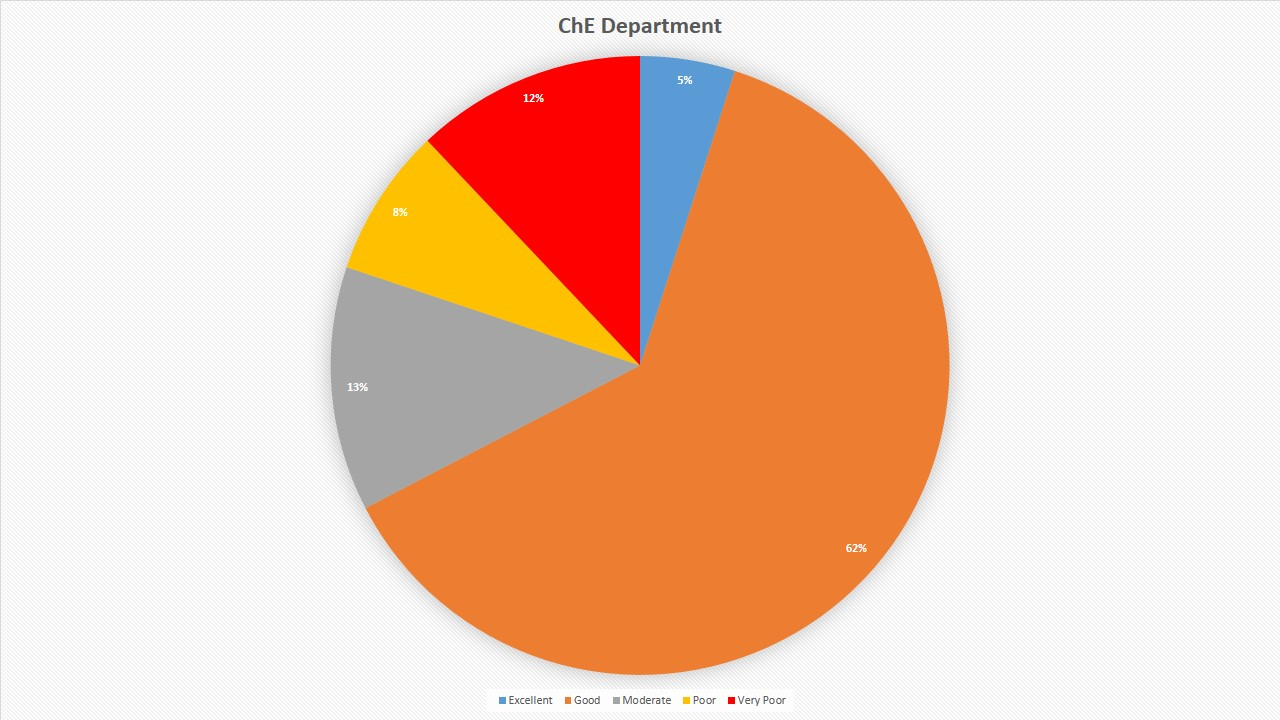
\includegraphics[width=\linewidth]{Figures/Slide8.jpg}
  \decoRule
  \caption[Performance of CHE Department]{Performance of CHE Department}
  \label{fig:Performance of CHE Department}
\end{figure}



\subsubsection{NAME Department}
The overall performance of NAME department is shown in Figure \ref{fig:Performance of NAME Department}.
\begin{table}
\caption{Performance of NAME Department}
\label{tab:name}
\centering
\begin{tabular}{|c| c| }
\toprule
\tabhead{Class Label} & \tabhead{Percent}\\
\midrule
Excellent & $8\%$\\
Good & $48\%$\\
Moderate & $27\%$\\
Poor & $10\%$\\
Very Poor & $7\%$\\

\bottomrule
\end{tabular}
\end{table}
According to our classifier the percentage of each class label of NAME department is shown in Table \ref{tab:name}

\begin{figure}
   \centering
  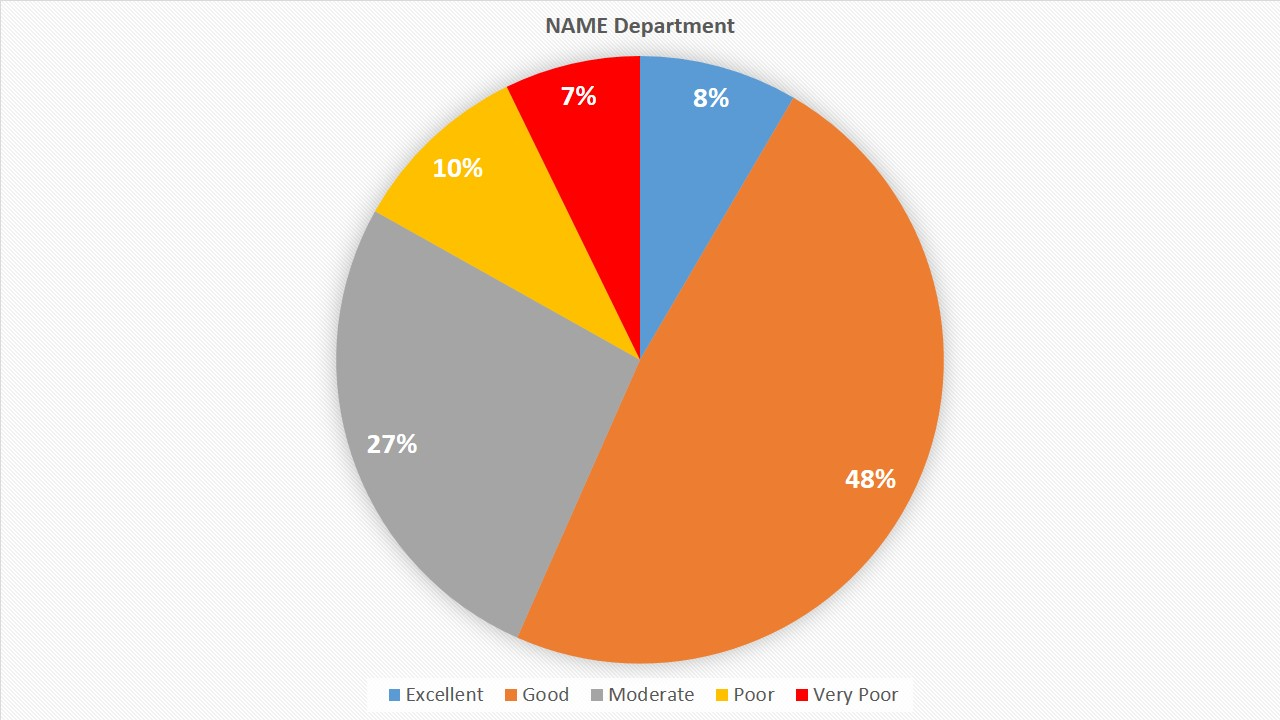
\includegraphics[width=\linewidth]{Figures/Slide9.jpg}
  \decoRule
  \caption[Performance of NAME Department]{Performance of NAME Department}
  \label{fig:Performance of NAME Department}
\end{figure}



\subsubsection{URP Department}
The overall performance of URP department is shown in Figure \ref{fig:Performance of URP Department}.
\begin{table}
\caption{Performance of URP Department}
\label{tab:urp}
\centering
\begin{tabular}{|c| c| }
\toprule
\tabhead{Class Label} & \tabhead{Percent}\\
\midrule
Excellent & $9\%$\\
Good & $40\%$\\
Moderate & $26\%$\\
Poor & $11\%$\\
Very Poor & $14\%$\\

\bottomrule
\end{tabular}
\end{table}
According to our classifier the percentage of each class label of URP department is shown in Table \ref{tab:urp}

\begin{figure}
   \centering
  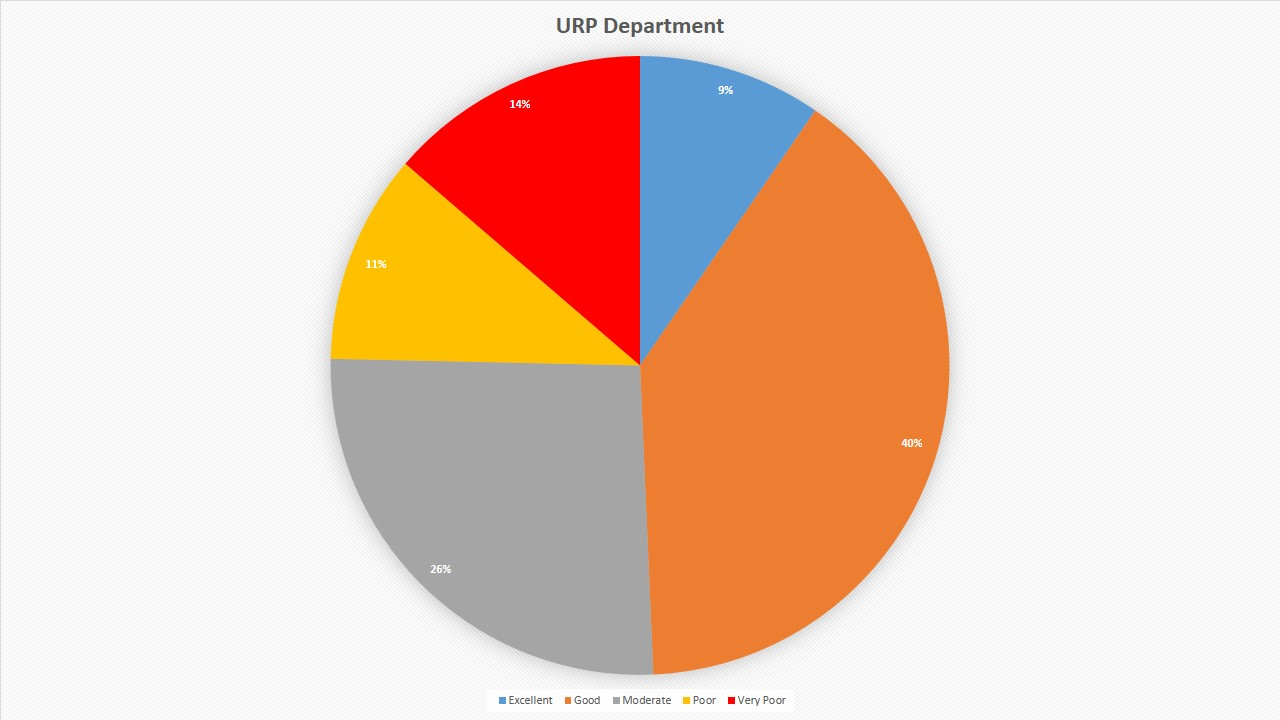
\includegraphics[width=\linewidth]{Figures/Slide10.jpg}
  \decoRule
  \caption[Performance of URP Department]{Performance of URP Department}
  \label{fig:Performance of URP Department}
\end{figure}





\subsubsection{ARCH Department}
The overall performance of ARCH department is shown in Figure \ref{fig:Performance of ARCH Department}.
\begin{table}
\caption{Performance of ARCH Department}
\label{tab:arch}
\centering
\begin{tabular}{|c| c| }
\toprule
\tabhead{Class Label} & \tabhead{Percent}\\
\midrule
Excellent & $2\%$\\
Good & $8\%$\\
Moderate & $32\%$\\
Poor & $16\%$\\
Very Poor & $39\%$\\

\bottomrule
\end{tabular}
\end{table}
According to our classifier the percentage of each class label of ARCH department is shown in Table \ref{tab:arch}

\begin{figure}
   \centering
  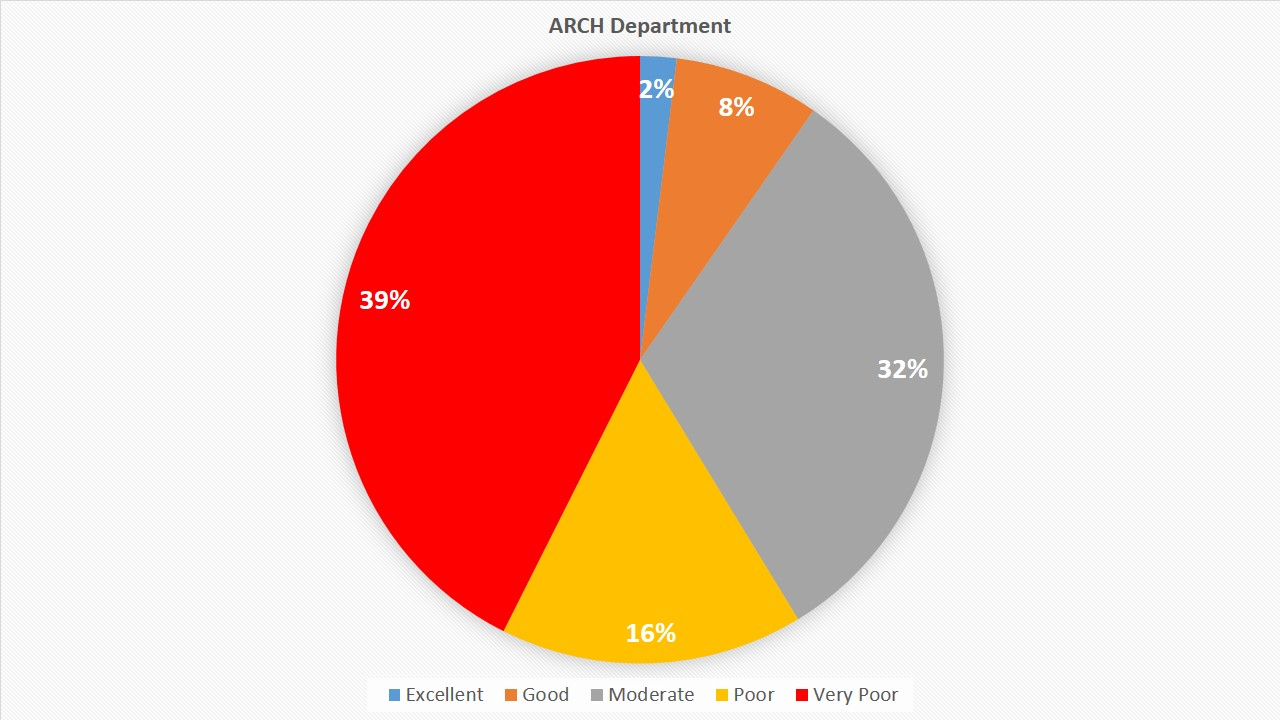
\includegraphics[width=\linewidth]{Figures/Slide11.jpg}
  \decoRule
  \caption[Performance of ARCH Department]{Performance of ARCH Department}
  \label{fig:Performance of ARCH Department}
\end{figure}




\subsubsection{WRE Department}
The overall performance of WRE department is shown in Figure \ref{fig:Performance of WRE Department}.
\begin{table}
\caption{Performance of WRE Department}
\label{tab:wre}
\centering
\begin{tabular}{|c| c| }
\toprule
\tabhead{Class Label} & \tabhead{Percent}\\
\midrule
Excellent & $8\%$\\
Good & $30\%$\\
Moderate & $35\%$\\
Poor & $12\%$\\
Very Poor & $15\%$\\

\bottomrule
\end{tabular}
\end{table}
According to our classifier the percentage of each class label of WRE department is shown in Table \ref{tab:wre}

\begin{figure}
   \centering
  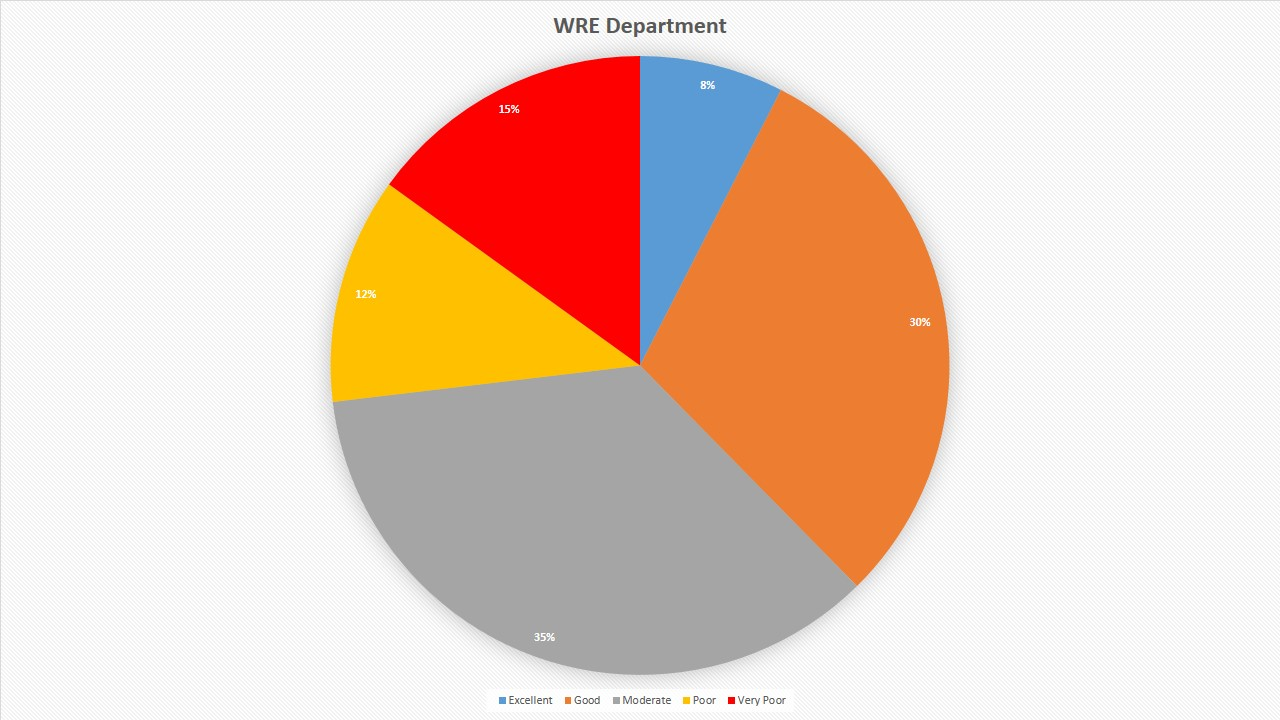
\includegraphics[width=\linewidth]{Figures/Slide12.jpg}
  \decoRule
  \caption[Performance of WRE Department]{Performance of WRE Department}
  \label{fig:Performance of WRE Department}
\end{figure}


 
% Chapter 1

\chapter{Conclusion} % Main chapter title

\label{Conclusion} % For referencing the chapter elsewhere, use \ref{Chapter1} 

%----------------------------------------------------------------------------------------

% Define some commands to keep the formatting separated from the content 

%----------------------------------------------------------------------------------------

\section{Summary of Thesis}
We used classification technique to discover knowledge from biis student data in this thesis project. All programming and necessary statistical analysis was done using java programming. The raw data set was full of impurities. So, we have to do an extensive amount of preprocessing on the data before applying it in our algorithm. Training data set was prepared very carefully and with logistic reasoning. The results of the classier was statistically analyzed and was stored in tabular form and graphical form for better visualization of the findings. The accuracy of the classifier is about 76\%. The low accuracy is due to the variations and impurities of the input data.   
%----------------------------------------------------------------------------------------

\section{General Findings}
The Classifier has five class labels. They are excellent,good,moderate,poor,very poor. After completing statistical analysis some major findings are
\begin{itemize}
\item EEE and CSE departments have a higher percentage in top levels. ARCH department has a higher percentage at the lowest level.

\item On average female students have better academic performance than male students.
\item Attached students dominate in the higher classes over the resident students.
\item Class Attendance and class attendance is very important for a student's overall performance.Students with good attendance trends to be in higher classes.
\item Class test marks are also very important for a student. Students with high percentage of class test marks trend to be in the higher classes. On the other hand students with lower percentage of class test marks fall in lower classes.

\end{itemize}


%----------------------------------------------------------------------------------------

\section{Future Works}

We used only classification rules to discover knowledge from data. In future we want to combine the clustering algorithm  with this one to get more accurate result.
\\The current accuracy is low. So we want to improve the accuracy by applying accuracy improvement algorithm.
\\We want to use this project to make a complete system for student evaluation.
  

%----------------------------------------------------------------------------------------

 

%----------------------------------------------------------------------------------------
%	THESIS CONTENT - APPENDICES
%----------------------------------------------------------------------------------------

\appendix % Cue to tell LaTeX that the following "chapters" are Appendices

% Include the appendices of the thesis as separate files from the Appendices folder
% Uncomment the lines as you write the Appendices

% Appendix A

\chapter{Appendix Title Here} % Main appendix title

\label{AppendixA} % For referencing this appendix elsewhere, use \ref{AppendixA}

Write your Appendix content here.
%% Appendix Template

\chapter{More Statistical Analysis Results} % Main appendix title

\label{Appendix B} % Change X to a consecutive letter; for referencing this appendix elsewhere, use \ref{AppendixX}

We also derived some statistical result from our processed data. This results is not related to our classifier.
Some of the results are discussed below 
\section{Department wise Different Grade Comparison}

\begin{figure}[H]
   \centering
  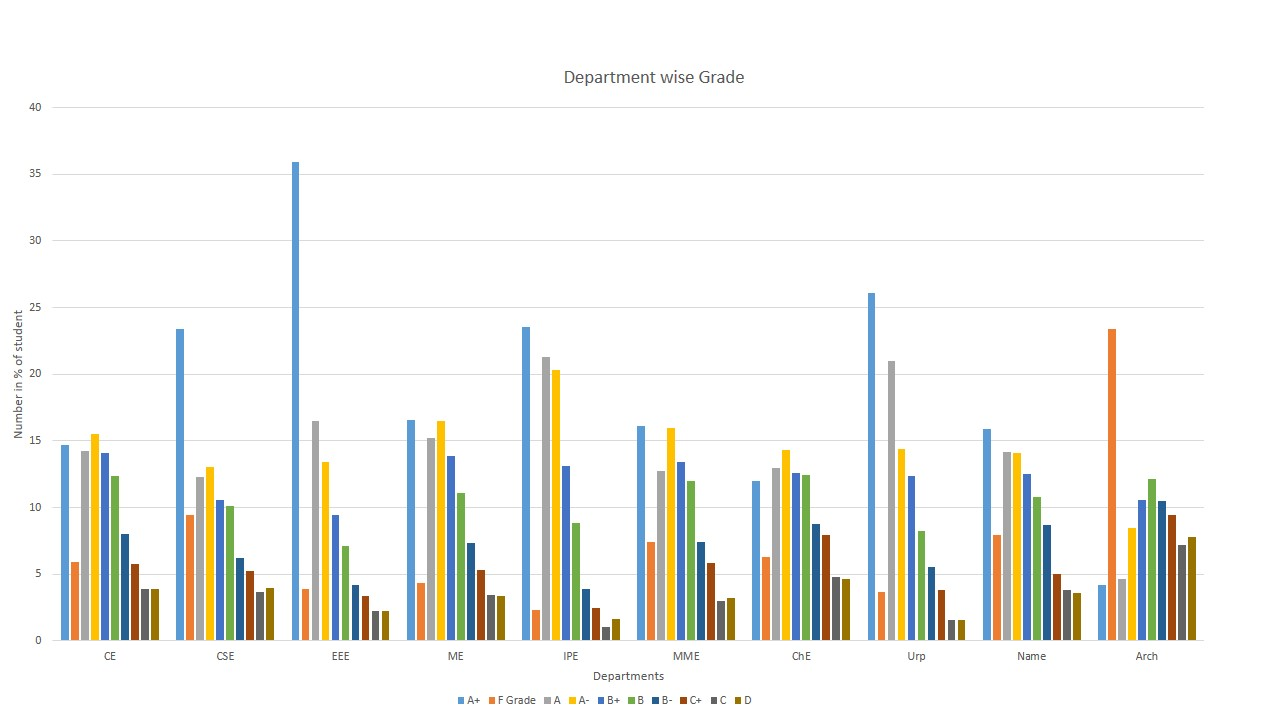
\includegraphics[width=\linewidth]{Figures/deptgrade.jpg}
  \decoRule
  \caption[Different Grades for Dept]{Different Grades for Dept}
  \label{fig:Different Grades for Dept}
\end{figure}

Figure \ref{fig:Different Grades for Dept} shows the frequency of different letter grades for different department.
For example students of EEE department get A+ more than other grades. On the other hand students of Architecture department get most percentage of F grade among other grades. 


\begin{figure}[H]
   \centering
  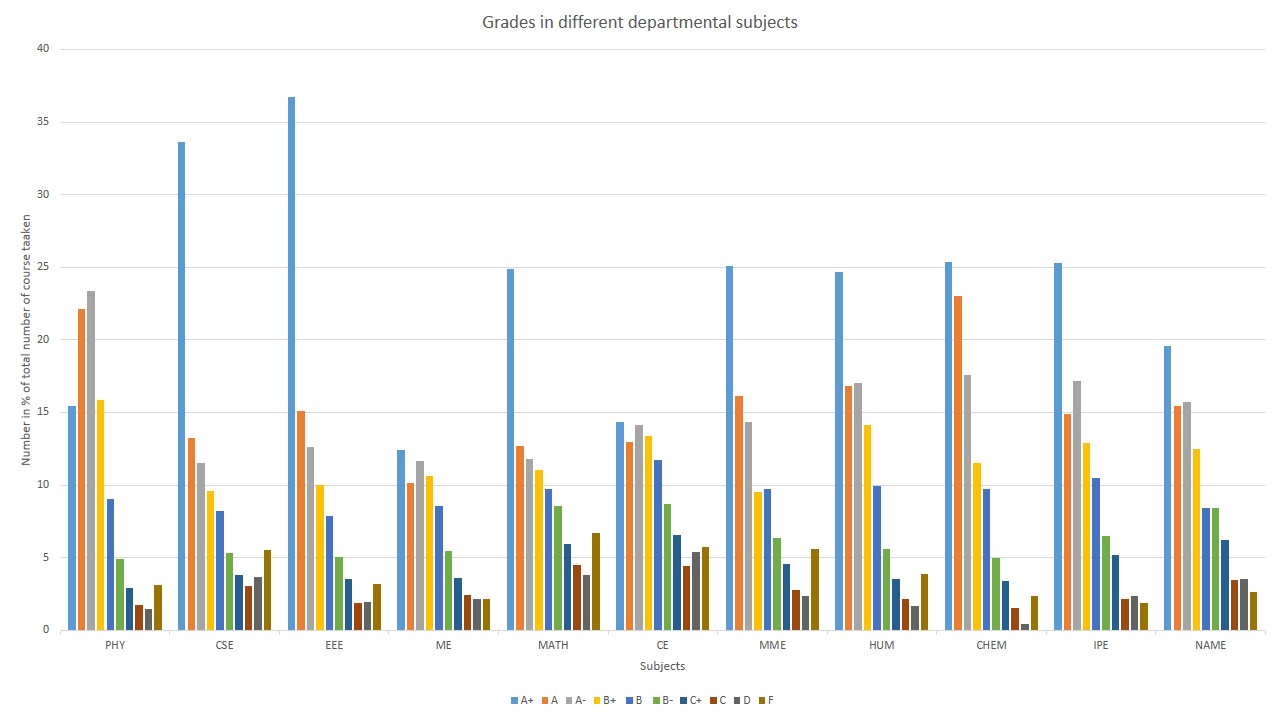
\includegraphics[width=\linewidth]{Figures/depresult.jpg}
  \decoRule
  \caption[Different Grades for Subjects]{Different Grades for Subjects}
  \label{fig:Different Grades for Subjects}
\end{figure}


Figure \ref{fig:Different Grades for Subjects} shows the frequency of grades in different departmental subjects.
As we can see students get most A+ in EEE subjects and get most F grade in MATH subjects.

%% Appendix Template

\chapter{Details of Department Name} % Main appendix title

\label{Appendix C} % Change X to a consecutive letter; for referencing this appendix elsewhere, use \ref{AppendixX}

EEE = Electrical and Electronics Engineering .\\
CSE = Computer Science and Engineering.\\
IPE = Industrial Production Engineering.\\
ME = Mechanical Engineering.\\
NAME = Naval Architecture and Marine Engineering.\\
ARCH = Architecture Department.\\
URP = Urban and Regional Planning.\\
WRE = Water Research Engineering.\\
CE = Civil Engineering.\\
ChE = Chemical Engineering.\\ 

%----------------------------------------------------------------------------------------
%	BIBLIOGRAPHY
%----------------------------------------------------------------------------------------

\printbibliography[heading=bibintoc]

%----------------------------------------------------------------------------------------

\end{document}  
